\subsection{Methodology}

A big part of the methodology that is used to solve the game requires the use of
backwards induction.
Backwards induction is a method that is used to solve a game by starting at the
terminal nodes and working backwards to the root node~\cite{watson2002strategy}.
The terminal nodes from Figure~\ref{fig:imperfect_info_game} are the nodes that
are connected to the choice of the distribution service.
In essence, by working backwards from the choice of the distribution service
and then to the choices of the queueing systems the game can be solved.
Furthermore, by finding the distribution's service response for all possible
pairs of strategies that the two queueing systems can choose from, the game can
be reduced to a two-player Normal form game.


\subsubsection{Distribution service and Brent's method}
\label{sec:best_response_distribution_service}

Form the distribution service's perspective all information are known and can be
used to find the best possible strategy to maximise their payoff.
In fact, having the two strategy choices of the two queueing systems the
distribution service can find the optimal strategy that satisfies
equation~(\ref{eq:obj_distributor_2}).
Consider the pair of strategies \((T_A^*, T_B^*)\) that correspond to a possible
strategy choice of queueing system A and queueing system B.
The distribution service can then find the best strategy by solving
equation~(\ref{eq:obj_distributor_2}) for \(T_A = T_A^*\) and \(T_B = T_B^*\).
This can be done by using Brent's method~\cite{brent_method}.

Brent's method is a root-finding algorithm which combines the bisection
method~\cite{corliss1977root}., the secant method~\cite{secantmethod} and
inverse quadratic interpolation~\cite{epperson2021introduction}.
The algorithm is used to find the root \(x^*\) of a function \(f(x)\) from
within the interval \([a, b]\) such that \(f(a) < f(x^*) < f(b)\).
Consider equation (\ref{eq:obj_distributor_2}).
Under the assumption that \(O(p_A; T_A, T_B)\) is either non-increasing or
non-decreasing in \(p_A\), the root can be found by using Brent's method
for \(p_A \in [0, 1]\).

\begin{equation*}
    O(p_A; T_A, T_B) = \alpha L_A(p_A) + (1 - \alpha) B_A(p_A) -
    \alpha L_B(1 - p_A) - (1 - \alpha)B_B(1 - p_A)
\end{equation*}

One of the requirements for Brent's method is \(f(a)f(b) < 0\).
In other words the function must change sign within the interval \([a, b]\).
For this particular scenario, the function \(f(p_A)\) needs to have a different
sign for \(f(p_A = 0)\) and \(f(p_A = 1)\).
In case \(f(a)f(b) \geq 0\), brent's algorithm cannot be used.
Instead, the value of \(p_A\) becomes:

\begin{equation}\label{eq:obj_distributor_no_brent_method}
    p_A = \begin{cases}
        1 & \text{if } f(0) < 0 \text{ and } f(1) < 0 \\
        0 & \text{if } f(0) > 0 \text{ and } f(1) > 0
    \end{cases}
\end{equation}

The first case of equation~(\ref{eq:obj_distributor_no_brent_method})
corresponds to the event where both \(f(0)\) and \(f(1)\) are negative.
Therefore, for all values of \(p_A \in [0, 1]\) the objective function is
negative, which means that:
\[
    \alpha L_A(p_A) + (1 - \alpha) B_A(p_A) <
    \alpha L_B(p_B) - (1 - \alpha) B_B(p_B), \quad \text{for all } p_A \in [0,1]
\]

Thus, the distribution service's best response would be to send all individuals
to queueing system A (\(p_A=1, p_B=0\)).
Similarly, the second case of
equation~(\ref{eq:obj_distributor_no_brent_method}) corresponds to the event
where for all values of \(p_A \in [0, 1]\) the objective function is
positive, which means that:
\[
    \alpha L_A(p_A) + (1 - \alpha) B_A(p_A) >
    \alpha L_B(p_B) - (1 - \alpha) B_B(p_B), \quad \text{for all } p_A \in [0,1]
\]
Equivalently, this indicates that the distribution service's best response
would be to send all individuals to queueing system B (\(p_A=0, p_B=1\)).
Therefore, the methodology that is used to find the best \(p_A\) that satisfies
equation~(\ref{eq:obj_distributor_2}) can by calculated in the following way:

\begin{equation}\label{eq:obj_distributor_implementation}
    p_A = \begin{cases}
        1, & \text{if } O(0) < 0 \text{ and } O(1) < 0 \\
        0, & \text{if } O(0) > 0 \text{ and } O(1) > 0 \\
        \text{Use Brent's method}, & \text{if } O(0)O(1) < 0
    \end{cases}
\end{equation}

where \(O(p_A)\) is the objective function of the distribution service described
in equation~(\ref{eq:obj_distributor_2}).

\paragraph{Examples}\label{sec:brent_method_example}
Consider a distribution service whose arrival rate of type 2 individuals is
\(\lambda_2 = 4\) and the `importance'-parameter is \(\alpha = 0.2\).
Additionally, let queueing system \(A\) and queueing system \(B\) have the
following parameters:

\begin{multicols}{2}
    \begin{itemize}
        \item \(\lambda_1^A = 2\)
        \item \(\mu^A = 3\)
        \item \(C^A = 3\)
        \item \(T^A = 8\)
        \item \(N^A = 15\)
        \item \(M^A = 10\)
        \item \(\lambda_1^B = 1\)
        \item \(\mu^B = 1\)
        \item \(C^B = 3\)
        \item \(T^B = 10\)
        \item \(N^B = 10\)
        \item \(M^B = 5\)
    \end{itemize}
\end{multicols}

The distribution service's best response for this particular example can be
found at the intersection of the two decision values of the two queueing
systems over \(p_A\).
Figure~\ref{fig:brent_method_example} illustrates the distribution service's
best response for this particular example.

\begin{figure}[H]
    \centering
    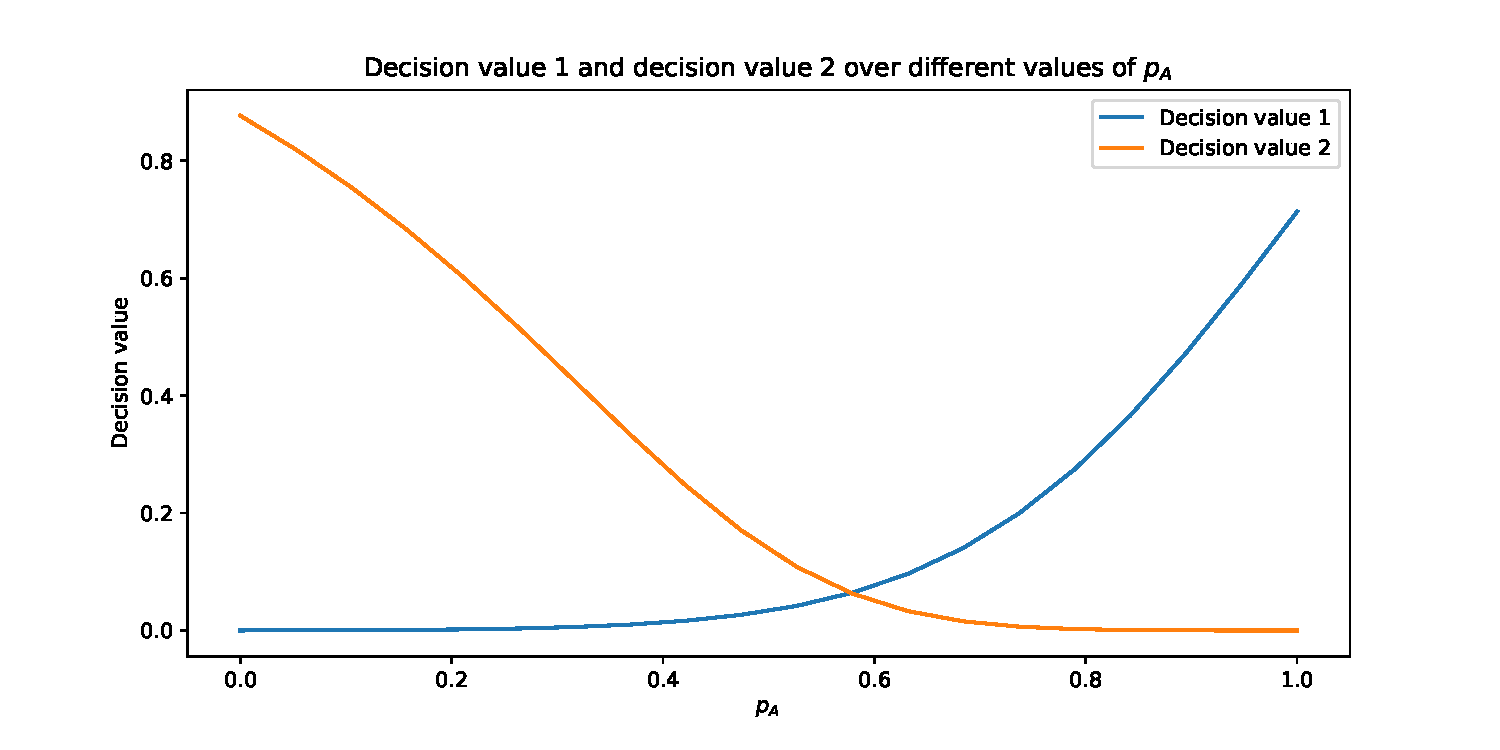
\includegraphics[width=\textwidth]{chapters/04_game_theoretic_model/img/brents_method/brent_method_example.pdf}
    \caption{Decision values for queueing system A and queueing system B}
    \label{fig:brent_method_example}
\end{figure}

In order to apply Brent's method to the current example the differences between
the two decision values need to be calculated.
Figure~\ref{fig:brent_method_diffs} shows that the value of \(p_A\) that the
distribution service should pick is where the function crosses the \(x\)-axis.

\begin{figure}[H]
    \centering
    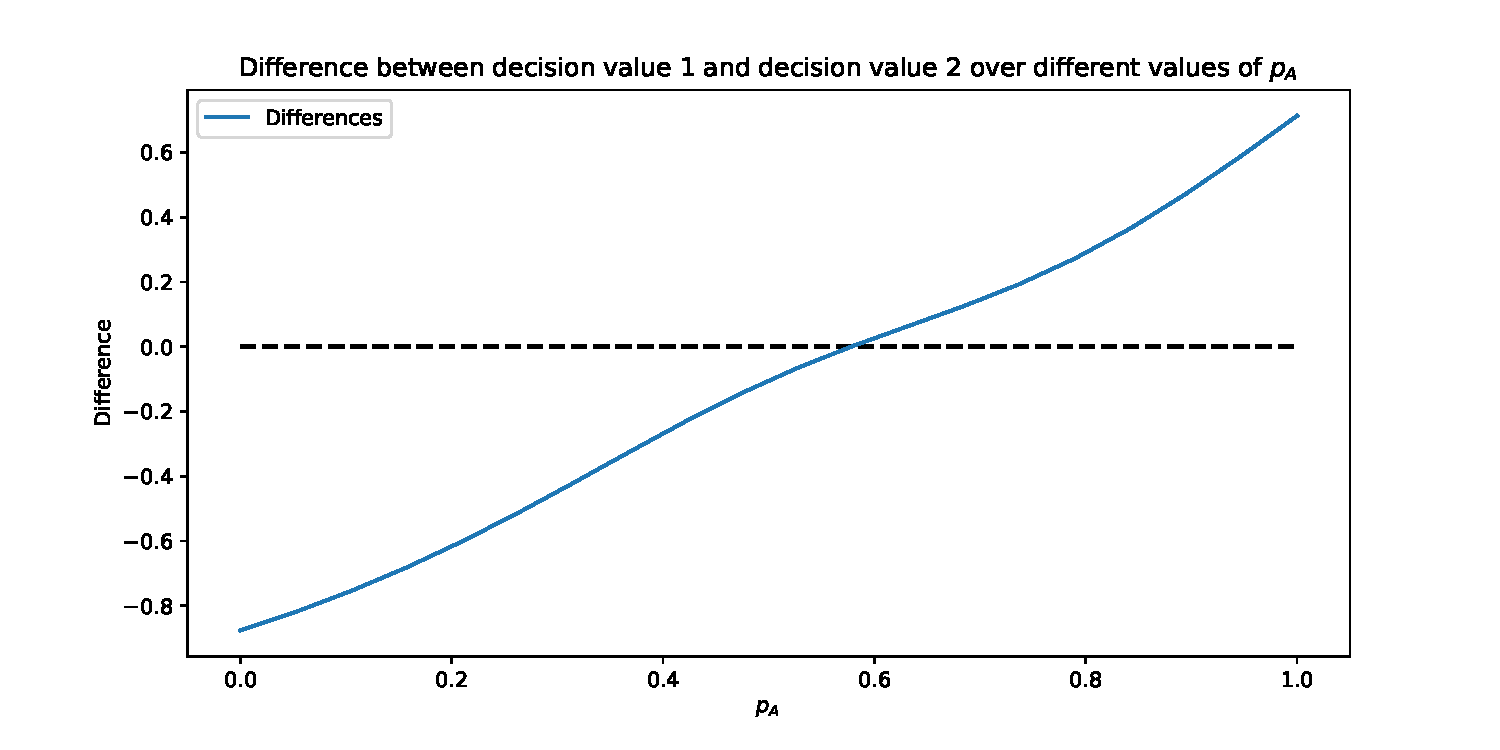
\includegraphics[width=\textwidth]{chapters/04_game_theoretic_model/img/brents_method/brent_method_diffs.pdf}
    \caption{Brent's method on the differences}
    \label{fig:brent_method_diffs}
\end{figure}

In fact, the value of \(p_A\) that the distribution service should pick, for
this particular example, is \(p_A = 0.58\).
That is the point in which the line of the difference between the two decision
values crosses the \(x\)-axis.

Consider now the same parameters as in the previous example, for different
values of the service rate of queueing system \(A\), \(\mu^A =
\{1,1.5,2,2.5,3\}\).

\begin{figure}[H]
    \centering
    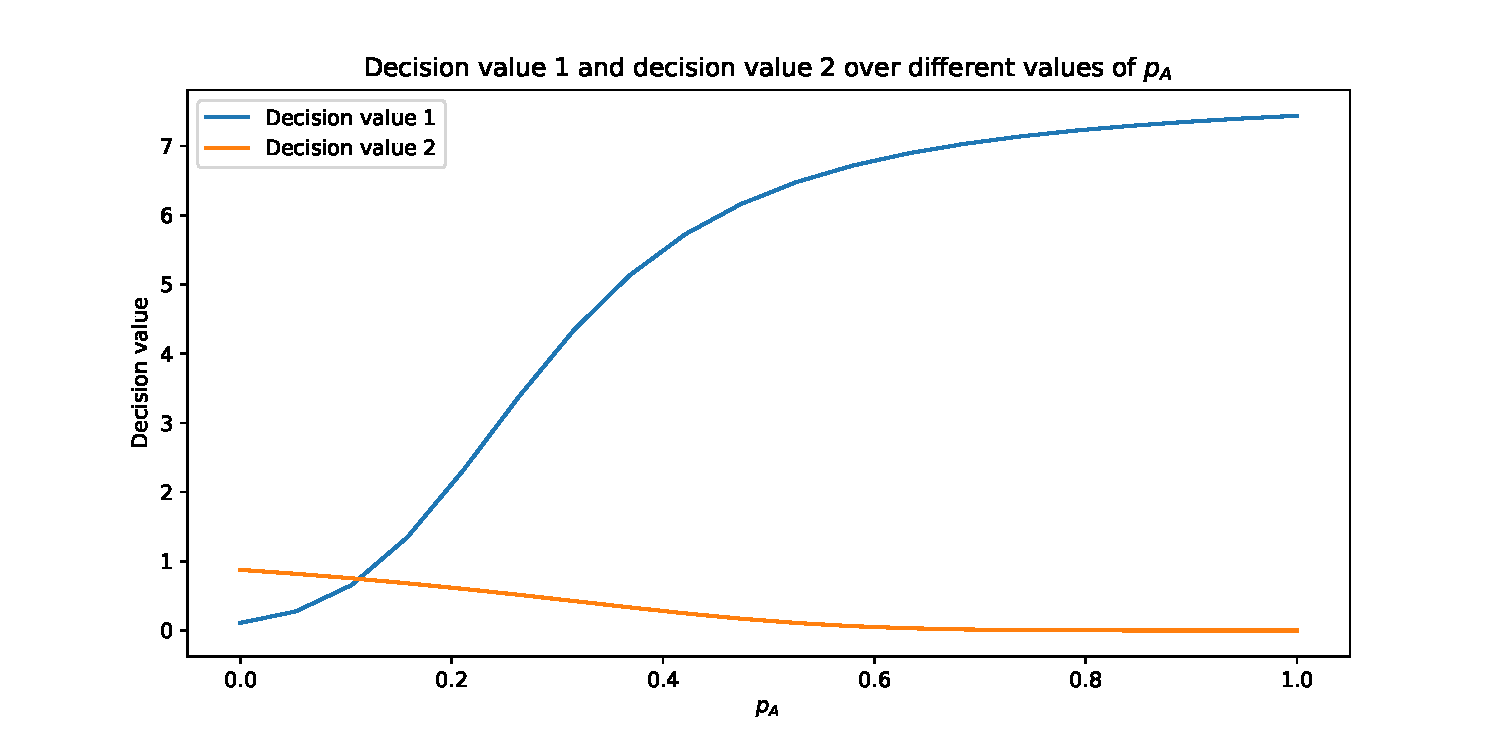
\includegraphics[width=\textwidth]{chapters/04_game_theoretic_model/img/brents_method/brent_method_example_mu_A_1.0.pdf}
    \caption{\(\mu^A = 1\)}
    \label{fig:brent_method_example_mu_A_1}
\end{figure}

\begin{figure}[H]
    \centering
    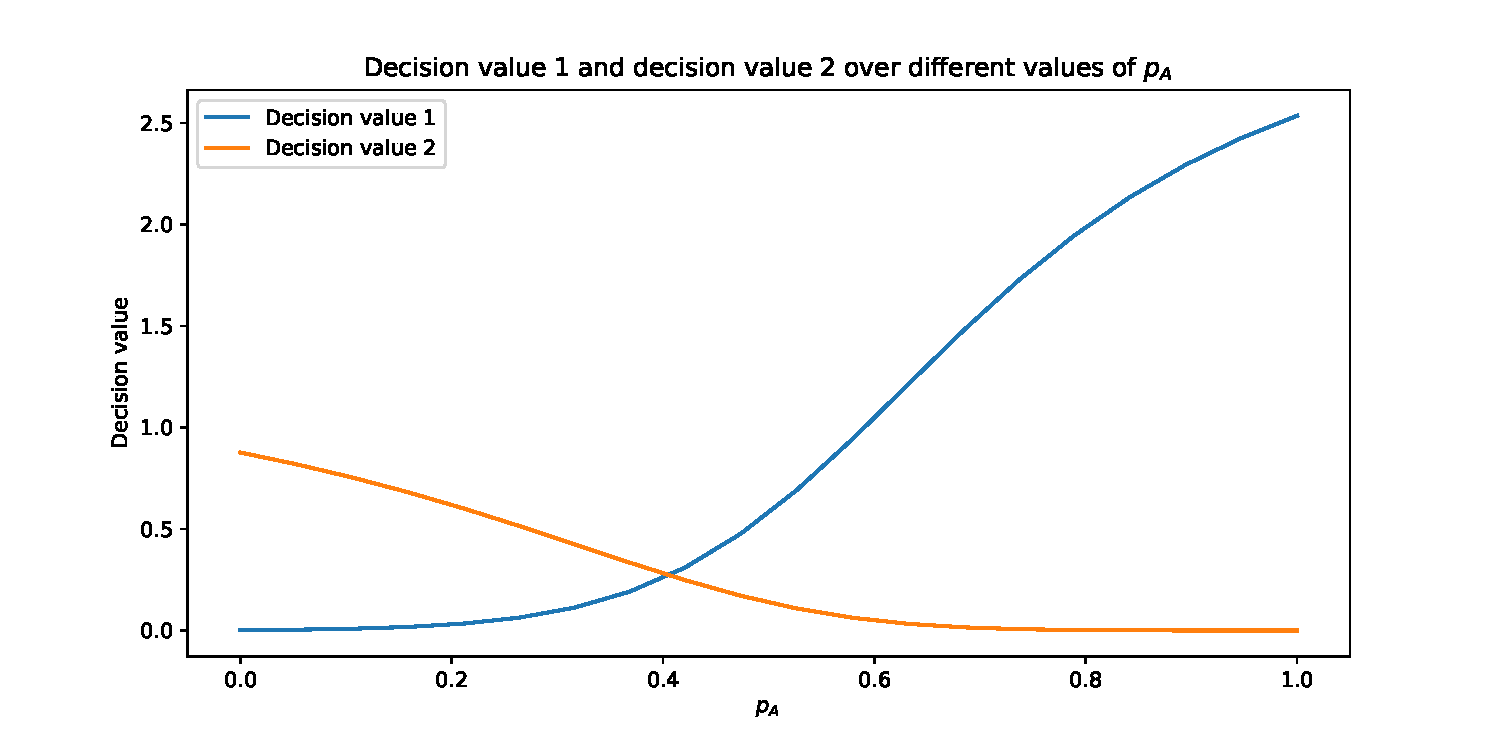
\includegraphics[width=\textwidth]{chapters/04_game_theoretic_model/img/brents_method/brent_method_example_mu_A_1.5.pdf}
    \caption{\(\mu^A = 1.5\)}
    \label{fig:brent_method_example_mu_A_2}
\end{figure}

\begin{figure}[H]
    \centering
    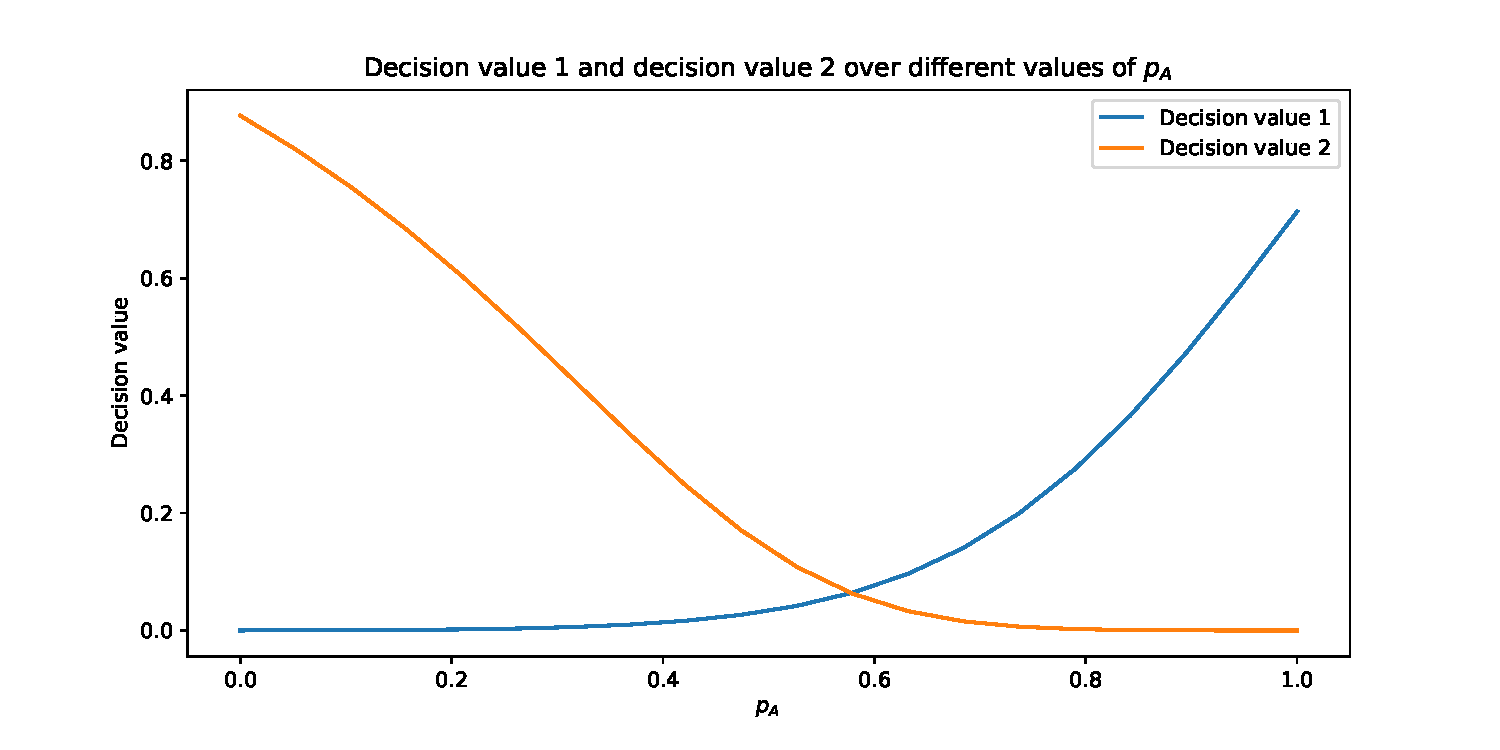
\includegraphics[width=\textwidth]{chapters/04_game_theoretic_model/img/brents_method/brent_method_example_mu_A_2.0.pdf}
    \caption{\(\mu^A = 2\)}
    \label{fig:brent_method_example_mu_A_3}
\end{figure}

\begin{figure}[H]
    \centering
    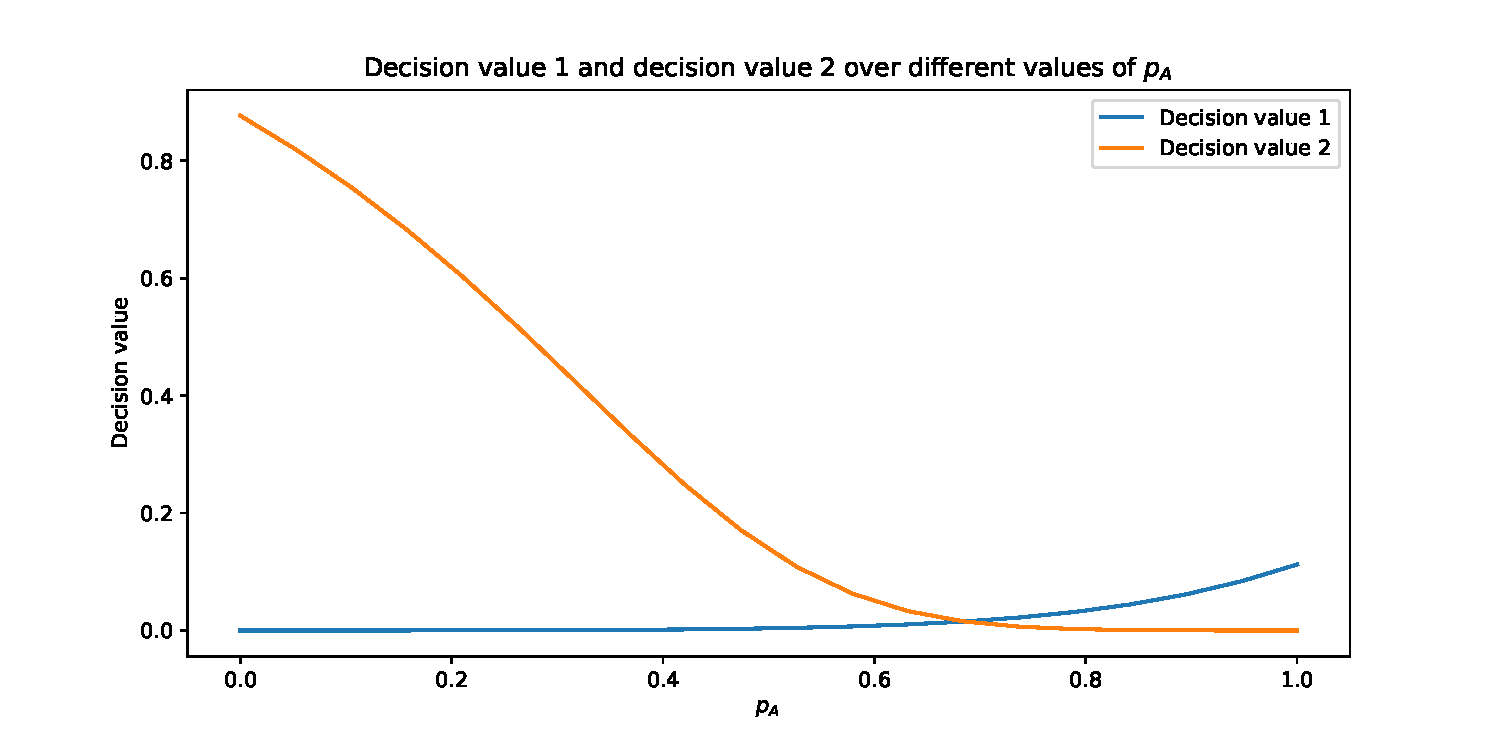
\includegraphics[width=\textwidth]{chapters/04_game_theoretic_model/img/brents_method/brent_method_example_mu_A_2.5.pdf}
    \caption{\(\mu^A = 2.5\)}
    \label{fig:brent_method_example_mu_A_4}
\end{figure}

\begin{figure}[H]
    \centering
    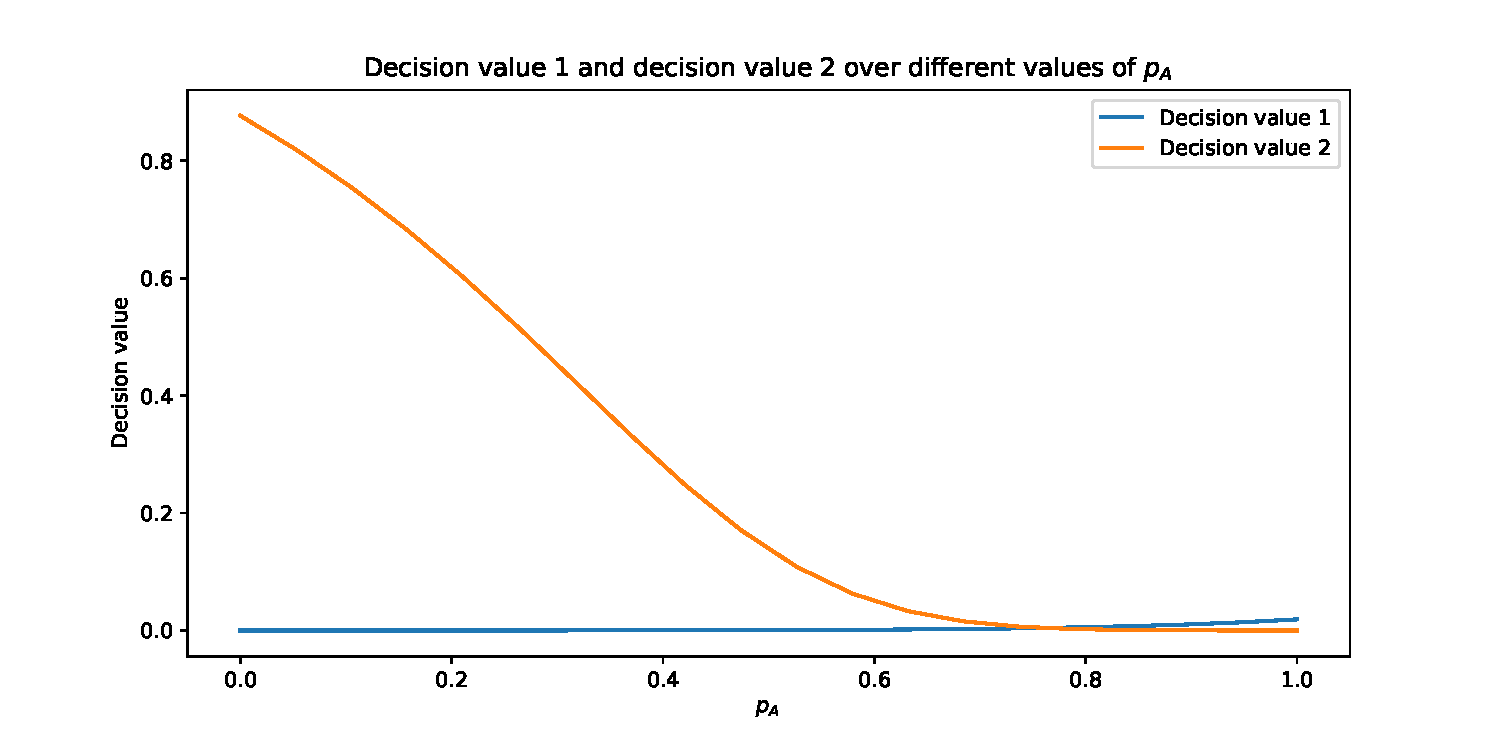
\includegraphics[width=\textwidth]{chapters/04_game_theoretic_model/img/brents_method/brent_method_example_mu_A_3.0.pdf}
    \caption{\(\mu^A = 3\)}
    \label{fig:brent_method_example_mu_A_5}
\end{figure}

It can be seen from Figures~\ref{fig:brent_method_example_mu_A_1} -
\ref{fig:brent_method_example_mu_A_5} that as the service rate of queueing
system \(A\) increases, the intersection point of the two decision values moves
from \(p_A=0\) towards \(p_A=1\).

In addition consider a different example with the same parameters as before
but by increasing the threshold of queueing system \(A\) from \(T^A = 8\) to
\(T^A = 10\) and decreasing the threshold of queueing system \(B\) from
\(T^B = 10\) to \(T^B = 2\).
Figure~\ref{fig:brent_method_special_case} shows the decision values that
correspond to the two queueing systems of the new example.

\begin{figure}[H]
    \centering
    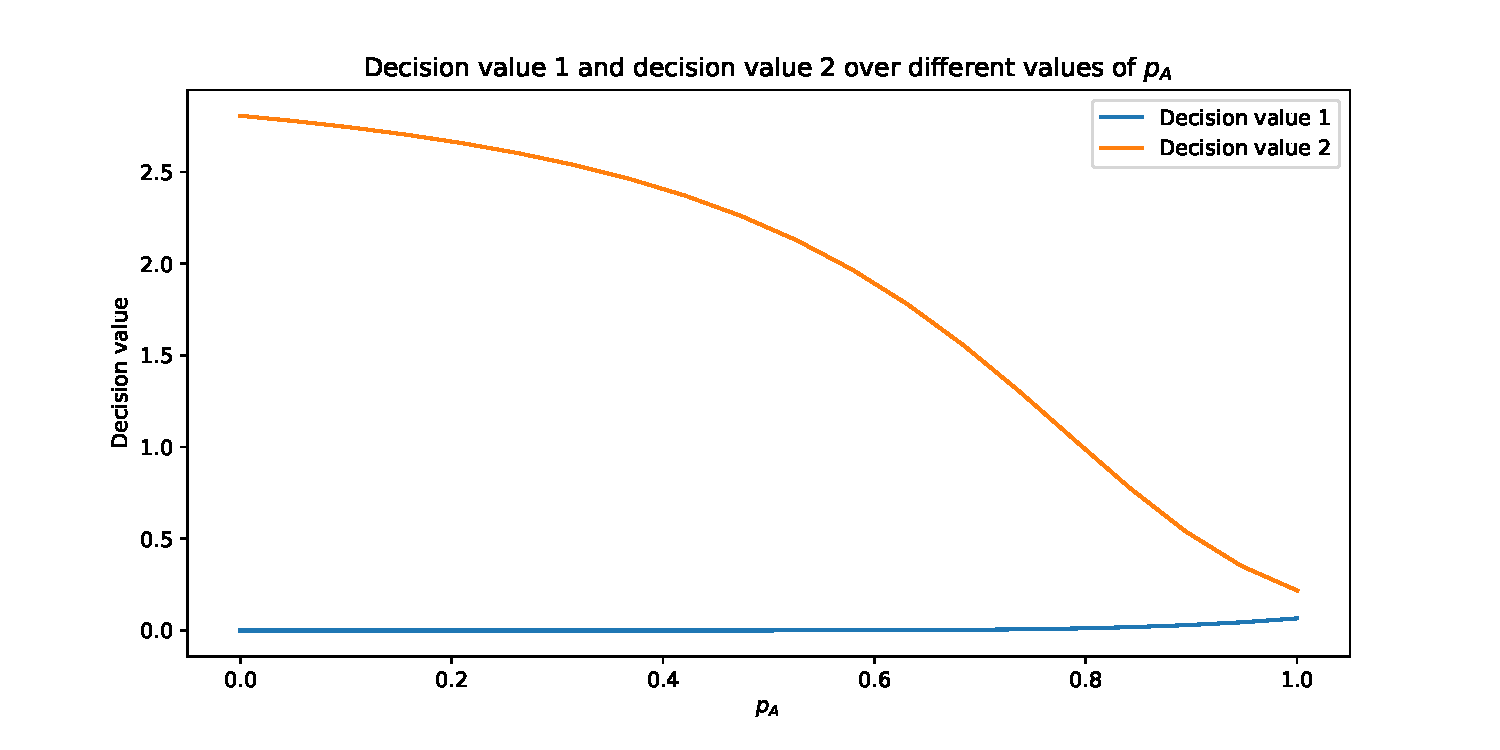
\includegraphics[width=\textwidth]{chapters/04_game_theoretic_model/img/brents_method/brent_method_special_case.pdf}
    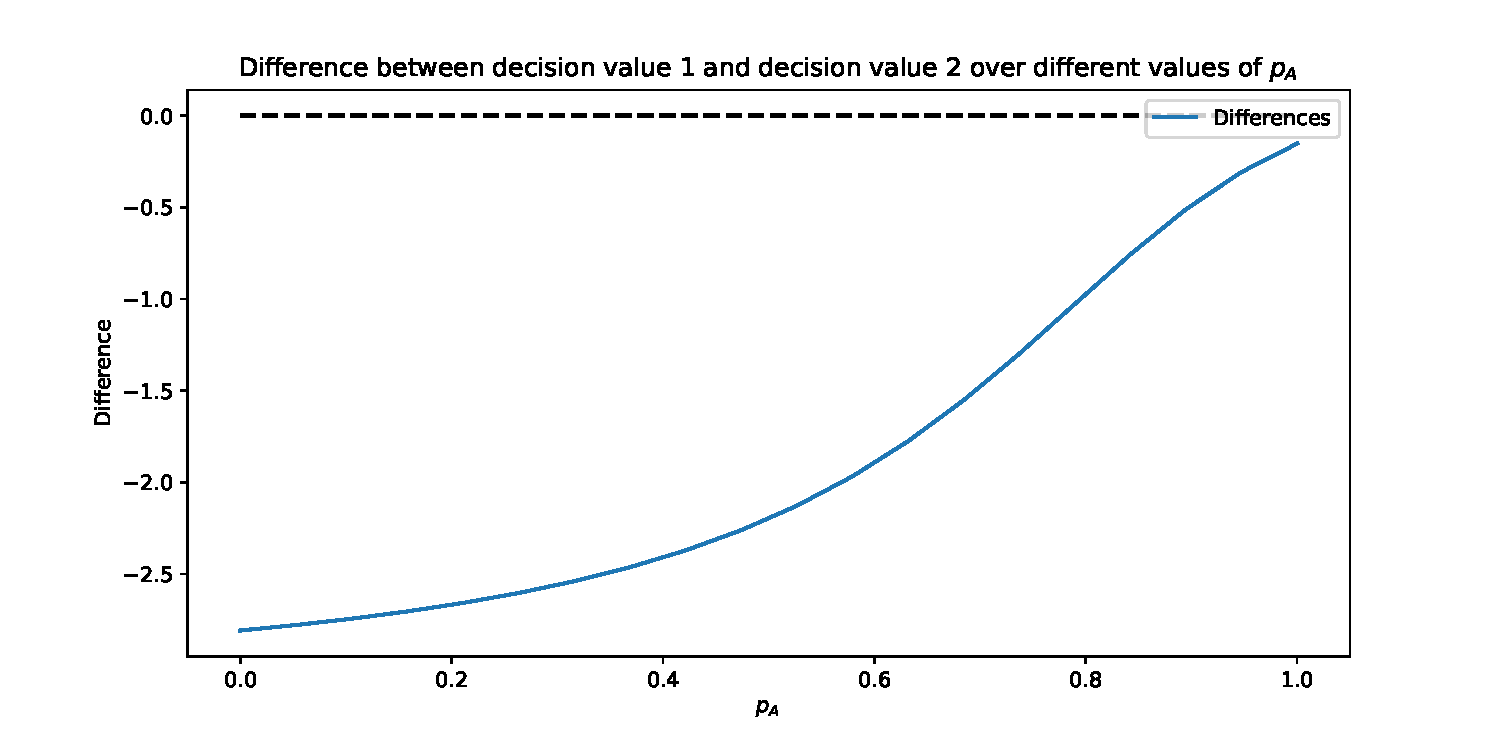
\includegraphics[width=\textwidth]{chapters/04_game_theoretic_model/img/brents_method/brent_method_special_case_diffs.pdf}
    \caption{Decision values for queueing system A and queueing system B}
    \label{fig:brent_method_special_case}
\end{figure}

It can be observed that for all values of \(p_A\) the decision value of queueing
system \(A\) is less than the decision value of queueing system \(B\).
Since the differences of them don't pass through the x-axis within the interval
\([0,1]\), Brent's method cannot be used since \(f(0)f(1) < 0\).
Therefore, using equation~(\ref{eq:obj_distributor_implementation}) the
distribution service's best response should be \(p_A = 1\).

\paragraph{Implementation}

The first part of the implementation of the distribution service's best
response is to calculate the difference between the decision values of the two
queueing systems.
Function \lstinline[style=pystyle]{get_mean_blocking_difference_using_markov}
is the python implementation of the first part of
equation~(\ref{eq:obj_distributor_2}).

\begin{lstlisting}[style=pystyle]
>>> import ambulance_game as abg
>>> def get_mean_blocking_difference_using_markov(
...     prop_1,
...     lambda_2,
...     lambda_1_1,
...     lambda_1_2,
...     mu_1,
...     mu_2,
...     num_of_servers_1,
...     num_of_servers_2,
...     threshold_1,
...     threshold_2,
...     system_capacity_1,
...     system_capacity_2,
...     buffer_capacity_1,
...     buffer_capacity_2,
...     alpha=0,
... ):
...     """
...     Get a weighted mean blocking difference between two systems. This
...     function is to be used as a routing function to find the point at
...     which it is set to 0. This function calculates:
...         - a*(1 - P(A_1)) + (1 - a)*B_1
...         - a*(1 - P(A_2)) + (1 - a)*B_2
...     and returns their difference.
...     Parameters
...     ----------
...     prop_1 : float
...         The proportion of class 2 individuals to distribute to the first
...         system
...     lambda_2 : float
...         The overall arrival rate of class 2 individuals for both systems
...     lambda_1_1 : float
...         The arrival rate of class 1 individuals in the first system
...     lambda_1_2 : float
...         The arrival rate of class 1 individuals in the second system
...     mu_1 : float
...     mu_2 : float
...     num_of_servers_1 : int
...     num_of_servers_2 : int
...     threshold_1 : int
...     threshold_2 : int
...     system_capacity_1 : int
...     system_capacity_2 : int
...     buffer_capacity_1 : int
...     buffer_capacity_2 : int
...     Returns
...     -------
...     float
...         The weighted mean difference between the decision values of the
...         two systems
...     """
...     lambda_2_1 = prop_1 * lambda_2
...     lambda_2_2 = (1 - prop_1) * lambda_2
...
...     mean_blocking_time_1 = abg.markov.get_mean_blocking_time_using_markov_state_probabilities(
...         lambda_2=lambda_2_1,
...         lambda_1=lambda_1_1,
...         mu=mu_1,
...         num_of_servers=num_of_servers_1,
...         threshold=threshold_1,
...         system_capacity=system_capacity_1,
...         buffer_capacity=buffer_capacity_1,
...     )
...     mean_blocking_time_2 = abg.markov.get_mean_blocking_time_using_markov_state_probabilities(
...         lambda_2=lambda_2_2,
...         lambda_1=lambda_1_2,
...         mu=mu_2,
...         num_of_servers=num_of_servers_2,
...         threshold=threshold_2,
...         system_capacity=system_capacity_2,
...         buffer_capacity=buffer_capacity_2,
...     )
...     prob_accept_1 = abg.markov.get_accepting_proportion_of_class_2_individuals(
...         lambda_1=lambda_1_1,
...         lambda_2=lambda_2_1,
...         mu=mu_1,
...         num_of_servers=num_of_servers_1,
...         threshold=threshold_1,
...         system_capacity=system_capacity_1,
...         buffer_capacity=buffer_capacity_1,
...     )
...     prob_accept_2 = abg.markov.get_accepting_proportion_of_class_2_individuals(
...         lambda_1=lambda_1_2,
...         lambda_2=lambda_2_2,
...         mu=mu_2,
...         num_of_servers=num_of_servers_2,
...         threshold=threshold_2,
...         system_capacity=system_capacity_2,
...         buffer_capacity=buffer_capacity_2,
...     )
...
...     decision_value_1 = (
...         alpha * (1 - prob_accept_1) + (1 - alpha) * mean_blocking_time_1
...     )
...     decision_value_2 = (
...         alpha * (1 - prob_accept_2) + (1 - alpha) * mean_blocking_time_2
...     )
...     return decision_value_1 - decision_value_2

\end{lstlisting}

Using the same example as in section~\ref{sec:brent_method_example} the
differences between the two decision values can be calculated using the next
code snippet.
Note, that the outcome of the function corresponds to the point of the line in
Figure~\ref{fig:brent_method_diffs} where \(p_A = 0.5\).

\begin{lstlisting}[style=pystyle]
>>> lambda_1_A = 2
>>> mu_A = 2
>>> num_of_servers_A = 3
>>> threshold_A = 8
>>> system_capacity_A = 15
>>> buffer_capacity_A = 10
>>> lambda_1_B = 1
>>> mu_B = 1
>>> num_of_servers_B = 3
>>> threshold_B = 10
>>> system_capacity_B = 10
>>> buffer_capacity_B = 5
>>>
>>> lambda_2 = 4
>>> alpha = 0.2
>>> p_A = 0.5
>>>
>>> get_mean_blocking_difference_using_markov(
...     prop_1=p_A,
...     lambda_2=lambda_2,
...     lambda_1_1=lambda_1_A,
...     lambda_1_2=lambda_1_B,
...     mu_1=mu_A,
...     mu_2=mu_B,
...     num_of_servers_1=num_of_servers_A,
...     num_of_servers_2=num_of_servers_B,
...     threshold_1=threshold_A,
...     threshold_2=threshold_B,
...     system_capacity_1=system_capacity_A,
...     system_capacity_2=system_capacity_B,
...     buffer_capacity_1=buffer_capacity_A,
...     buffer_capacity_2=buffer_capacity_B,
...     alpha=alpha,
... )
-0.10424302454312097

\end{lstlisting}

In addition function
\lstinline[style=pystyle]{calculate_class_2_individuals_best_response} uses
an implementation of Brent's method, implemented by the
\lstinline[style=pystyle]{scipy} library, to find the point at which the
difference between the two decision values is set to 0.

\begin{lstlisting}[style=pystyle]
>>> import scipy.optimize
>>> def calculate_class_2_individuals_best_response(
...     lambda_2,
...     lambda_1_1,
...     lambda_1_2,
...     mu_1,
...     mu_2,
...     num_of_servers_1,
...     num_of_servers_2,
...     threshold_1,
...     threshold_2,
...     system_capacity_1,
...     system_capacity_2,
...     buffer_capacity_1,
...     buffer_capacity_2,
...     lower_bound=0.01,
...     upper_bound=0.99,
...     alpha=0,
...     xtol=1e-04,
...     rtol=8.9e-16,
... ):
...     """
...     Obtains the optimal distribution of class 2 individuals such that the
...     blocking times in the two systems are identical and thus minimised.
...     The brentq function is used which is an algorithm created to find the
...     root of a function that combines root bracketing, bisection, and
...     inverse quadratic interpolation. In this specific example the root to
...     be found is the difference between the blocking times of two systems.
...     In essence the brentq algorithm attempts to find the value of prop_1
...     where the difference is zero.
...
...     Parameters
...     ----------
...     lower_bound : float, optional
...         The lower bound of p_1, by default 0.01
...     upper_bound : float, optional
...         The upper bound of p_1, by default 0.99
...     routing_function : function, optional
...         The function to find the root of
...     Returns
...     -------
...     float
...         The value of p_1 such that routing_function = 0
...     """
...
...     routing_function = get_mean_blocking_difference_using_markov
...     check_1 = routing_function(
...         prop_1=lower_bound,
...         lambda_2=lambda_2,
...         lambda_1_1=lambda_1_1,
...         lambda_1_2=lambda_1_2,
...         mu_1=mu_1,
...         mu_2=mu_2,
...         num_of_servers_1=num_of_servers_1,
...         num_of_servers_2=num_of_servers_2,
...         threshold_1=threshold_1,
...         threshold_2=threshold_2,
...         system_capacity_1=system_capacity_1,
...         system_capacity_2=system_capacity_2,
...         buffer_capacity_1=buffer_capacity_1,
...         buffer_capacity_2=buffer_capacity_2,
...         alpha=alpha,
...     )
...     check_2 = routing_function(
...         prop_1=upper_bound,
...         lambda_2=lambda_2,
...         lambda_1_1=lambda_1_1,
...         lambda_1_2=lambda_1_2,
...         mu_1=mu_1,
...         mu_2=mu_2,
...         num_of_servers_1=num_of_servers_1,
...         num_of_servers_2=num_of_servers_2,
...         threshold_1=threshold_1,
...         threshold_2=threshold_2,
...         system_capacity_1=system_capacity_1,
...         system_capacity_2=system_capacity_2,
...         buffer_capacity_1=buffer_capacity_1,
...         buffer_capacity_2=buffer_capacity_2,
...         alpha=alpha,
...     )
...
...     if check_1 >= 0 and check_2 >= 0:
...         return 0
...     if check_1 <= 0 and check_2 <= 0:
...         return 1
...
...     brentq_arguments = (
...         lambda_2,
...         lambda_1_1,
...         lambda_1_2,
...         mu_1,
...         mu_2,
...         num_of_servers_1,
...         num_of_servers_2,
...         threshold_1,
...         threshold_2,
...         system_capacity_1,
...         system_capacity_2,
...         buffer_capacity_1,
...         buffer_capacity_2,
...         alpha,
...     )
...
...     optimal_split = scipy.optimize.brentq(
...         routing_function,
...         a=lower_bound,
...         b=upper_bound,
...         args=brentq_arguments,
...         xtol=xtol,
...         rtol=rtol,
...     )
...     return optimal_split

\end{lstlisting}

The next piece of code uses
function~\lstinline[style=pystyle]{calculate_class_2_individuals_best_response}
to find the optimal split of class 2 individuals between the two queueing
systems.
The same set of parameters are used as in the example in
Section~\ref{sec:brent_method_example}.
Note that this is the value of \(p_A\) for which the line of
Figure~\ref{fig:brent_method_diffs} crosses the \(x\)-axis.

\begin{lstlisting}[style=pystyle]
>>> calculate_class_2_individuals_best_response(
...     lambda_2=lambda_2,
...     lambda_1_1=lambda_1_A,
...     lambda_1_2=lambda_1_B,
...     mu_1=mu_A,
...     mu_2=mu_B,
...     num_of_servers_1=num_of_servers_A,
...     num_of_servers_2=num_of_servers_B,
...     threshold_1=threshold_A,
...     threshold_2=threshold_B,
...     system_capacity_1=system_capacity_A,
...     system_capacity_2=system_capacity_B,
...     buffer_capacity_1=buffer_capacity_A,
...     buffer_capacity_2=buffer_capacity_B,
...     alpha=alpha,
... )
0.5778494982926555

\end{lstlisting}


\subsubsection{Routing Matrix}

Section~\ref{sec:brent_method_example} showed how Brent's method can be used to
find the best response of the distribution service given the pair of strategies
played by the queueing systems \((T_A, T_B)\).
In order to properly solve the game, best response of the distribution service
needs to be calculated for every possible pair of strategies.
In essence, one needs to find the values of \(p_A\) and \(p_B\) that correspond
to every pair of \((T_A, T_B)\), and then use these values to construct the
routing matrix.
The routing matrix holds the values \((p_A, p_B)\) which are the proportion
of type 2 individuals to send to queueing systems \(A\) and \(B\).
Each pair \((p_A, p_B)\) can be calculated using
equation~(\ref{eq:obj_distributor_penalty}), as shown in
Section~\ref{sec:brent_method_example}, for all possible pairs of thresholds.
Thus, the routing matrix is a \(N_A \times N_B\) matrix, where \(N_A\) and
\(N_B\) are the capacities of Node 1 for queueing systems \(A\) and \(B\),
respectively.

\begin{equation}\label{eq:routing_matrix}
    R =
    \begin{pmatrix}
        (p_{1,1}^A, p_{1,1}^B) & (p_{1,2}^A, p_{1,2}^B) & \dots &
        (p_{1,N_B}^A, p_{1,N_B}^B) \\
        (p_{2,1}^A, p_{2,1}^B) & (p_{2,2}^A, p_{2,2}^B) & \dots &
        (p_{2,N_B}^A, p_{2,N_B}^B) \\
        \vdots & \vdots & \ddots & \vdots \\
        (p_{N_A,1}^A, p_{N_A,1}^B) & (p_{N_A,2}^A, p_{N_A,2}^B) & \dots &
        (p_{N_A,N_B}^A, p_{N_A,N_B}^B) \\
    \end{pmatrix}
\end{equation}

Note that since \(p_{i,j}^A + p_{i,j}^B = 1\) the routing matrix needs only to
store one of the two values; either \(p_{i,j}^A\) or \(p_{i,j}^B\).
Thus, the routing matrix \(R\) can be simplified to:

\begin{equation}\label{eq:routing_matrix_simplified}
    R =
    \begin{pmatrix}
        p_{1,1}^A & p_{1,2}^A & \dots & p_{1,N_B}^A \\
        p_{2,1}^A & p_{2,2}^A & \dots & p_{2,N_B}^A \\
        \vdots & \vdots & \ddots & \vdots \\
        p_{N_A,1}^A & p_{N_A,2}^A & \dots & p_{N_A,N_B}^A \\
    \end{pmatrix}
\end{equation}


\paragraph{Example}\label{sec:routing_matrix_example}
Using the same example as in Section~\ref{sec:brent_method_example}, the routing
matrix can be calculated by finding the values of \(p_A\) and \(p_B\) for every
possible pair of thresholds \((T_A, T_B)\).
The arrival rate of type 2 individuals is arrival rate of type 2 individuals is
\(\lambda_2 = 4\) and the `importance'-parameter is \(\alpha = 0.2\).
The remaining parameters that relate to the two queueing systems are as follows:

\begin{multicols}{2}
    \begin{itemize}
        \item \(\lambda_1^A = 2\)
        \item \(\mu^A = 3\)
        \item \(C^A = 3\)
        \item \(N^A = 15\)
        \item \(M^A = 10\)
        \item \(\lambda_1^B = 1\)
        \item \(\mu^B = 1\)
        \item \(C^B = 3\)
        \item \(N^B = 10\)
        \item \(M^B = 5\)
    \end{itemize}
\end{multicols}

Note that the thresholds are not defined for the routing matrix since they are
not constants.
In fact the thresholds can take values from 1 to \(N_i\) for each queueing
system.
Thus, \(T^A \in \{1, 2, \dots, 15\}\) and \(T^B \in \{1, 2, \dots, 10\}\).
The routing matrix is then going to be a \(15 \times 10\) matrix where each
entry \(i, j\) consists of the best response of the distribution service when
\(Q_A\) plays a strategy of \(T_A=i\) and \(Q_B\) plays a strategy of \(T_B=j\).


\begin{equation*}
    R =
    \begin{pmatrix}
        0.59 & 0.22 & 0.16 & 0.15 & 0.15 & 0.15 & 0.15 & 0.14 & 0.13 & 0.06 \\
        0.94 & 0.67 & 0.51 & 0.49 & 0.47 & 0.46 & 0.45 & 0.44 & 0.41 & 0.31 \\
        1.00 & 0.85 & 0.71 & 0.67 & 0.64 & 0.62 & 0.60 & 0.57 & 0.54 & 0.45 \\
        1.00 & 0.86 & 0.74 & 0.70 & 0.67 & 0.64 & 0.62 & 0.60 & 0.57 & 0.48 \\
        1.00 & 0.88 & 0.76 & 0.72 & 0.69 & 0.67 & 0.64 & 0.62 & 0.59 & 0.51 \\
        1.00 & 0.89 & 0.78 & 0.74 & 0.71 & 0.68 & 0.66 & 0.64 & 0.61 & 0.54 \\
        1.00 & 0.90 & 0.79 & 0.75 & 0.72 & 0.70 & 0.68 & 0.66 & 0.63 & 0.56 \\
        1.00 & 0.91 & 0.81 & 0.77 & 0.74 & 0.71 & 0.69 & 0.67 & 0.64 & 0.58 \\
        1.00 & 0.91 & 0.82 & 0.78 & 0.75 & 0.73 & 0.71 & 0.68 & 0.66 & 0.59 \\
        1.00 & 0.92 & 0.83 & 0.80 & 0.76 & 0.74 & 0.72 & 0.70 & 0.67 & 0.61 \\
        1.00 & 0.93 & 0.84 & 0.80 & 0.77 & 0.75 & 0.73 & 0.71 & 0.68 & 0.62 \\
        1.00 & 0.93 & 0.85 & 0.81 & 0.78 & 0.76 & 0.74 & 0.72 & 0.69 & 0.64 \\
        1.00 & 0.95 & 0.87 & 0.83 & 0.80 & 0.78 & 0.75 & 0.73 & 0.71 & 0.65 \\
        1.00 & 0.98 & 0.90 & 0.86 & 0.83 & 0.80 & 0.78 & 0.76 & 0.73 & 0.68 \\
        1.00 & 1.00 & 0.99 & 0.94 & 0.90 & 0.87 & 0.84 & 0.82 & 0.79 & 0.74
    \end{pmatrix}    
\end{equation*}

Note that the entries of the routing matrix correspond to different pairs of
thresholds \((T_A, T_B)\).
In other words, the entry \(R_{i,j}\) corresponds to the pair \((T_A=i,T_B=j)\).
For example, consider the example discussed in
Section~\ref{sec:brent_method_example} that had the same set of parameters with
thresholds \(T_A=8, T_B=10\).
The best response of the distribution service is calculated to be \(p_A=0.58\)
and it can also be found in the routing matrix at the \(8^{th}\) row and
\(10^{th}\) column (i.e. \(R_{8,10} = 0.58\)).


\paragraph{Implementation}

The following function shows how the routing matrix can be calculated by using
function~\lstinline[style=pystyle]{calculate_class_2_individuals_best_response}
for every possible pair of thresholds.

\begin{lstlisting}[style=pystyle]
>>> import itertools
>>> import numpy as np
>>> def get_routing_matrix(
...    lambda_2,
...    lambda_1_1,
...    lambda_1_2,
...    mu_1,
...    mu_2,
...    num_of_servers_1,
...    num_of_servers_2,
...    system_capacity_1,
...    system_capacity_2,
...    buffer_capacity_1,
...    buffer_capacity_2,
...    alpha=0,
... ):
...    """
...    Get the optimal distribution matrix that consists of the proportion of
...    individuals to be distributed to each hospital for all possible
...    combinations of thresholds of the two hospitals (T_1, T_2). For every
...    set of thresholds, the function fills the entries of the matrix using
...    the proportion of individuals to distribute to hospital 1.
...
...    Parameters
...    ----------
...    lambda_2 : float
...    lambda_1_1 : float
...    lambda_1_2 : float
...    mu_1 : float
...    mu_2 : float
...    num_of_servers_1 : int
...    num_of_servers_2 : int
...    system_capacity_1 : int
...    system_capacity_2 : int
...    buffer_capacity_1 : int
...    buffer_capacity_2 : int
...    routing_function : function, optional
...        The function to use to get the optimal distribution of patients
...    Returns
...    -------
...    numpy array
...        The matrix with proportions of all possible combinations of
...        threshold
...    """
...    routing_matrix = np.zeros((system_capacity_1, system_capacity_2))
...    for threshold_1, threshold_2 in itertools.product(
...        range(1, system_capacity_1 + 1), range(1, system_capacity_2 + 1)
...    ):
...        opt = calculate_class_2_individuals_best_response(
...            lambda_2=lambda_2,
...            lambda_1_1=lambda_1_1,
...            lambda_1_2=lambda_1_2,
...            mu_1=mu_1,
...            mu_2=mu_2,
...            num_of_servers_1=num_of_servers_1,
...            num_of_servers_2=num_of_servers_2,
...            system_capacity_1=system_capacity_1,
...            system_capacity_2=system_capacity_2,
...            buffer_capacity_1=buffer_capacity_1,
...            buffer_capacity_2=buffer_capacity_2,
...            threshold_1=threshold_1,
...            threshold_2=threshold_2,
...            alpha=alpha,
...        )
...        routing_matrix[threshold_1 - 1, threshold_2 - 1] = opt
...    return routing_matrix

\end{lstlisting}

\begin{sloppypar}
Using the same set of parameters as in the example discussed in
Section~\ref{sec:routing_matrix_example}, the routing matrix can be calculated.
\end{sloppypar}

\begin{lstlisting}[style=pystyle]
>>> get_routing_matrix(
...    lambda_2=lambda_2,
...    lambda_1_1=lambda_1_A,
...    lambda_1_2=lambda_1_B,
...    mu_1=mu_A,
...    mu_2=mu_B,
...    num_of_servers_1=num_of_servers_A,
...    num_of_servers_2=num_of_servers_B,
...    system_capacity_1=system_capacity_A,
...    system_capacity_2=system_capacity_B,
...    buffer_capacity_1=buffer_capacity_A,
...    buffer_capacity_2=buffer_capacity_B,
...    alpha=alpha,
... )
array([[0.58864276, 0.22335975, 0.15533059, 0.15265663, 0.15078926,
        0.14922469, 0.14719237, 0.14271416, 0.12874758, 0.06396441],
       [0.93574605, 0.67443129, 0.51051637, 0.48986689, 0.474517  ,
        0.46234589, 0.45136222, 0.43786699, 0.41004722, 0.31135186],
       [1.        , 0.84928478, 0.70944125, 0.66945048, 0.63960878,
        0.61601954, 0.59573161, 0.5746382 , 0.54157719, 0.44625113],
       [1.        , 0.86430904, 0.73661752, 0.69683427, 0.66686909,
        0.64296716, 0.62233703, 0.6011736 , 0.56942852, 0.48372486],
       [1.        , 0.8769602 , 0.75856893, 0.71911699, 0.68913141,
        0.66505568, 0.64416384, 0.62297243, 0.59220666, 0.51352681],
       [1.        , 0.88782106, 0.77691989, 0.73780511, 0.7078792 ,
        0.68366777, 0.66270079, 0.64146588, 0.61149112, 0.5382421 ],
       [1.        , 0.89728669, 0.79261746, 0.75382586, 0.72401867,
        0.69978202, 0.6787237 , 0.65751624, 0.6282157 , 0.55939581],
       [1.        , 0.90564353, 0.80614796, 0.7677999 , 0.73815484,
        0.71398819, 0.69284969, 0.67167208, 0.64301254, 0.5778495 ],
       [1.        , 0.91312427, 0.81813225, 0.78016576, 0.75073204,
        0.72662301, 0.70549771, 0.68440782, 0.65624748, 0.59425681],
       [1.        , 0.91997634, 0.82894698, 0.79141059, 0.76218245,
        0.73812947, 0.71705972, 0.69606716, 0.66837977, 0.60914055],
       [1.        , 0.92662384, 0.83917256, 0.80200443, 0.77297551,
        0.74903033, 0.7279936 , 0.70708275, 0.67987751, 0.62310053],
       [1.        , 0.93417364, 0.85009707, 0.81320876, 0.7843084 ,
        0.7604156 , 0.73937585, 0.7185154 , 0.69171265, 0.63719748],
       [1.        , 0.94615952, 0.8654791 , 0.82845358, 0.79936661,
        0.77525057, 0.75399993, 0.73296783, 0.70639403, 0.65395543],
       [1.        , 0.97522952, 0.89772397, 0.85877431, 0.82812693,
        0.80267354, 0.78024478, 0.75829045, 0.73124439, 0.68050787],
       [1.        , 1.        , 0.98966703, 0.94066708, 0.90265479,
        0.87136701, 0.84412235, 0.81814844, 0.78822172, 0.73774973]])

\end{lstlisting}


\paragraph{Brent's method - tolerance sensitivity analysis}
\label{sec:brent_tolerance}

The implementation of Brent's method is being done using the
function~\lstinline[style=pystyle]{brentq}
from~\lstinline[style=pystyle]{SciPy}.
The function receives two essential arguments; another function for
which to find the root of, and the interval in which the root is located.
In addition to these two arguments, the function also receives two optional
arguments; \lstinline[style=pystyle]{xtol} and
\lstinline[style=pystyle]{rtol}~\cite{2020SciPy-NMeth}.
These two parameters are the ones that define the tolerance of the algorithm.
In other words, the smaller the tolerance parameters are, the more accurate
the result will be.
However, the smaller the tolerance parameters are, the more iterations will
be needed to find the root.
Therefore, the tolerance parameters are a trade-off between accuracy and
computation time.

The documentation of the~\lstinline[style=pystyle]{brentq} function states
that the default values of the tolerance parameters are
\lstinline[style=pystyle]{xtol=2e-12} and
\lstinline[style=pystyle]{rtol=8.881784197001252e-16}.
Within the the~\lstinline[style=pystyle]{brentq} function these two parameters
are used to ensure that
\lstinline[style=pystyle]{allclose(x, x0, atol=xtol, rtol=rtol) = True}.
Function \lstinline[style=pystyle]{allclose} is implemented by the
\lstinline[style=pystyle]{numpy} library~\cite{harris2020array}.
and checks if two arrays are element-wise similar given a certain tolerance.
The way the internal mechanisms of the~\lstinline[style=pystyle]{allclose}
function work is that given two values \(a\) and \(b\), with some absolute
tolerance (atol) and relative tolerance (rtol) parameters, the function returns
\lstinline[style=pystyle]{True} if:

\begin{equation}
    |a - b| \leq (\text{atol} + \text{rtol} \times |b|)
\end{equation}

These tolerance parameters are the once used by Brent's method to determine
if the root has been found.
In the remainder of this subsection the effect of the absolute tolerance
parameter \lstinline[style=pystyle]{xtol} will be analysed.
To determine the effect of the absolute tolerance parameters on the accuracy and
computation time of Brent's method, the method was ran for different set of
parameters and different values of the absolute tolerance parameter.
The two parameter sets that were used for these experiments are:

\begin{center}
    \small
    \begin{tabular}{||c|c|c|c|c|c|c|c|c|c|c|c|c||}
        \hline
        \(\lambda_2\) & \(\lambda_1^A\) & \(\lambda_1^B\) & \(T^A\) & \(T^B\) &
        \(\mu^A\) & \(\mu^B\) & \(C^A\) & \(C^B\) & \(N^A\) & \(N^B\) & \(M^A\) &
        \(M^B\) \\
        \hline\hline
        4 & 3 & 3 & 4 & 5 & 4 & 3 & 2 & 3 & [8,25] & 8 & 8 & 8 \\
        \hline
        5 & 2 & 2 & 7 & 10 & 3 & 2 & 3 & 4 & [7,24] & 15 & 10 & 10 \\
        \hline
    \end{tabular}
\end{center}
    
Note the system capacity of queueing system A varies for both parameter sets.
For every value of \(N_A\) Brent's algorithm was run for different values of
the absolute tolerance parameter \lstinline[style=pystyle]{xtol}.
The values of the absolute tolerance parameter that were used are:
\lstinline[style=pystyle]
{xtol = [1e-10, 1e-9, 1e-8, 1e-7, 1e-6, 1e-5, 0.0001, 0.001, 0.01, 0.1]}.
For each value of the absolute tolerance parameter, the algorithm was run 200
times and the computation time was recorded for each run.


\begin{figure}[H]
    \centering
    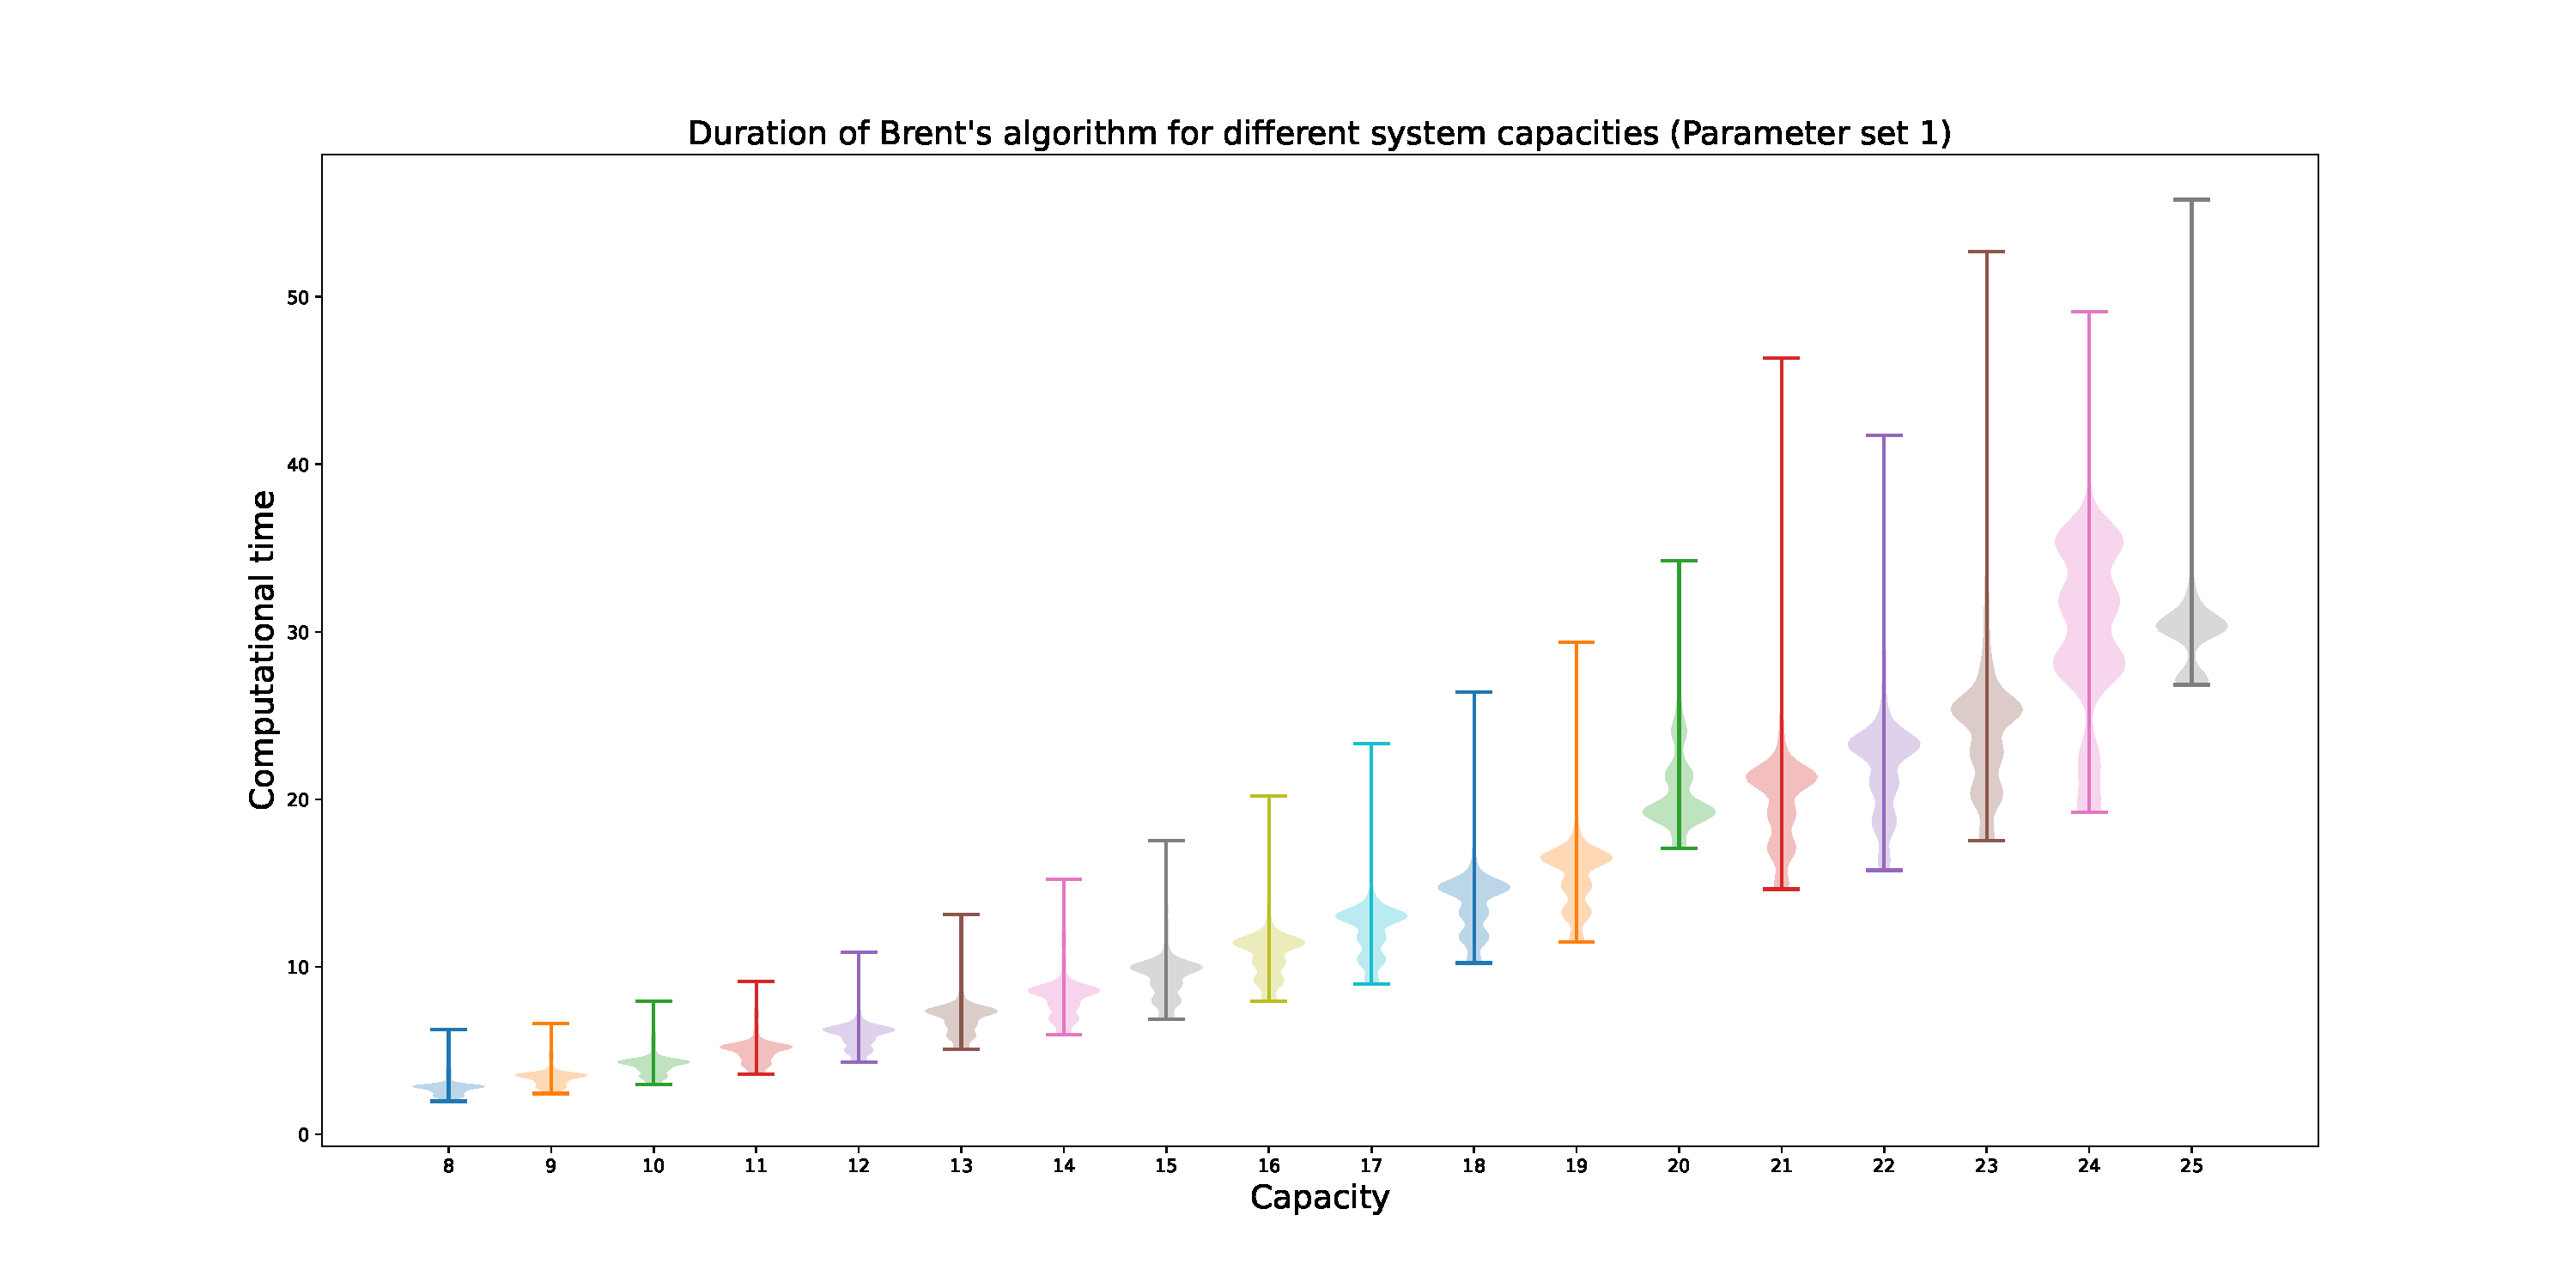
\includegraphics[width=\textwidth]{chapters/04_game_theoretic_model/img/brents_method/tolerance/tolerance_violinplots_1.pdf}
    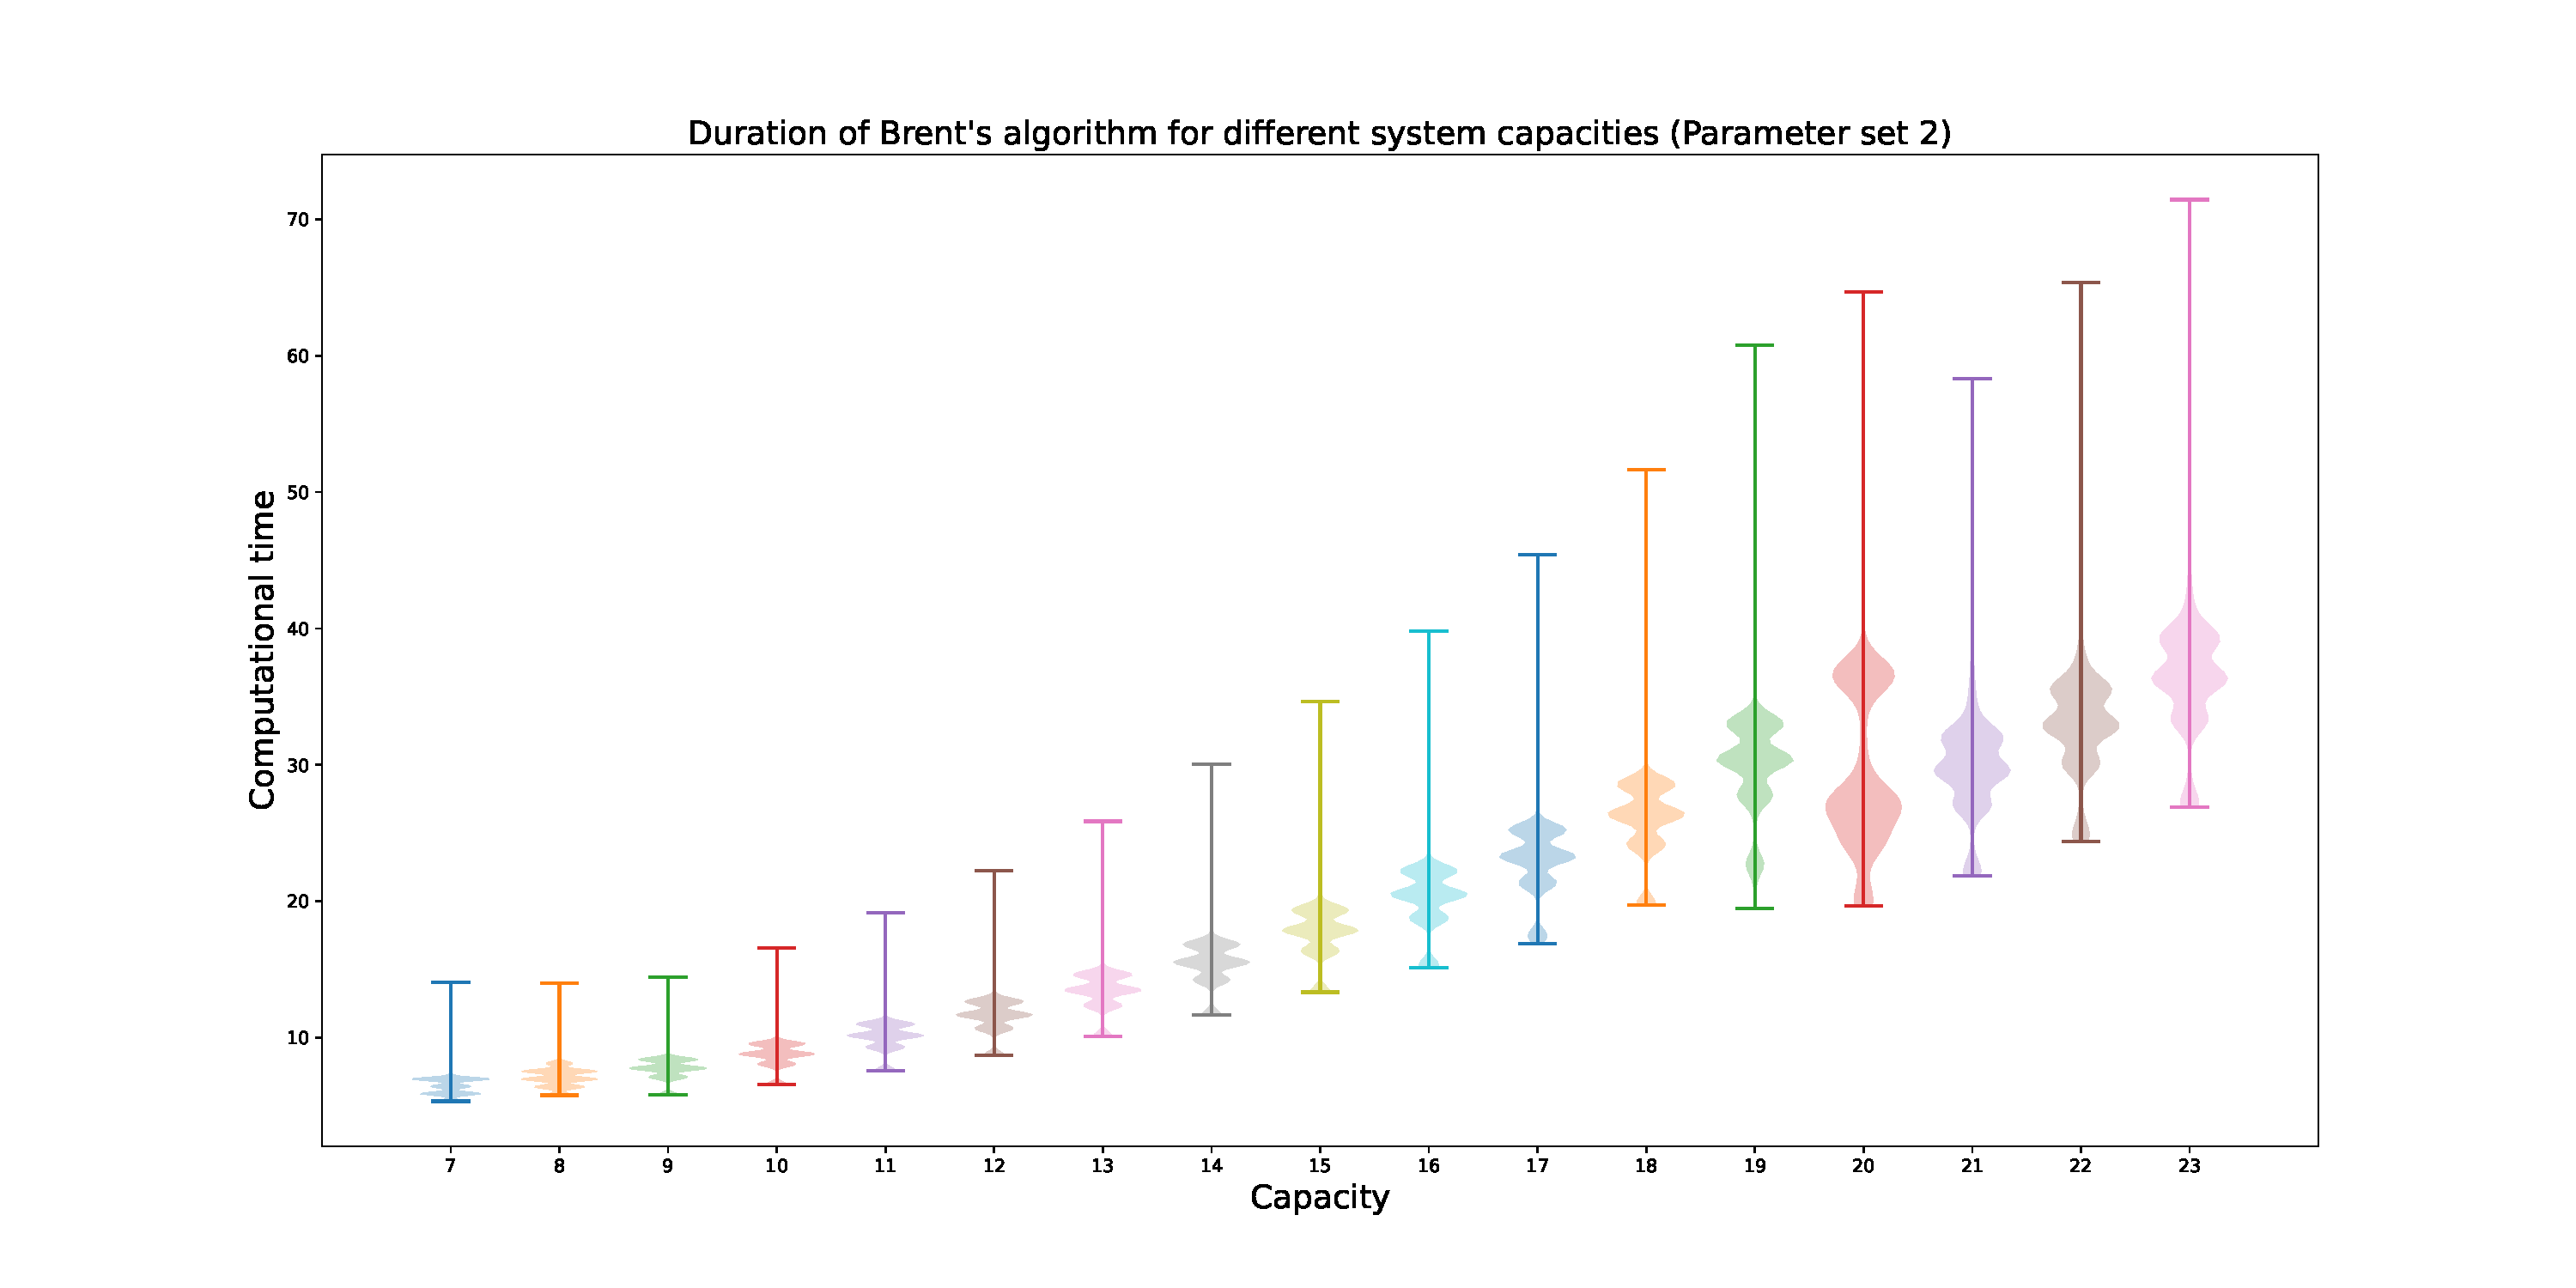
\includegraphics[width=\textwidth]{chapters/04_game_theoretic_model/img/brents_method/tolerance/tolerance_violinplots_2.pdf}
    \caption{
        Violinplots of the duration of Brent's method for different values of
        \(N_A\).
    }
    \label{fig:tolerance_violinplots}
\end{figure}

It can be seen that for both parameter sets in
Figure~\ref{fig:tolerance_violinplots} the duration of the algorithm is
increasing as \(N^A\) increases.
Note that the violinplots include all values of the tolerance parameters
\lstinline[style=pystyle]{xtol} that were used.

\begin{figure}[H]
    \centering
    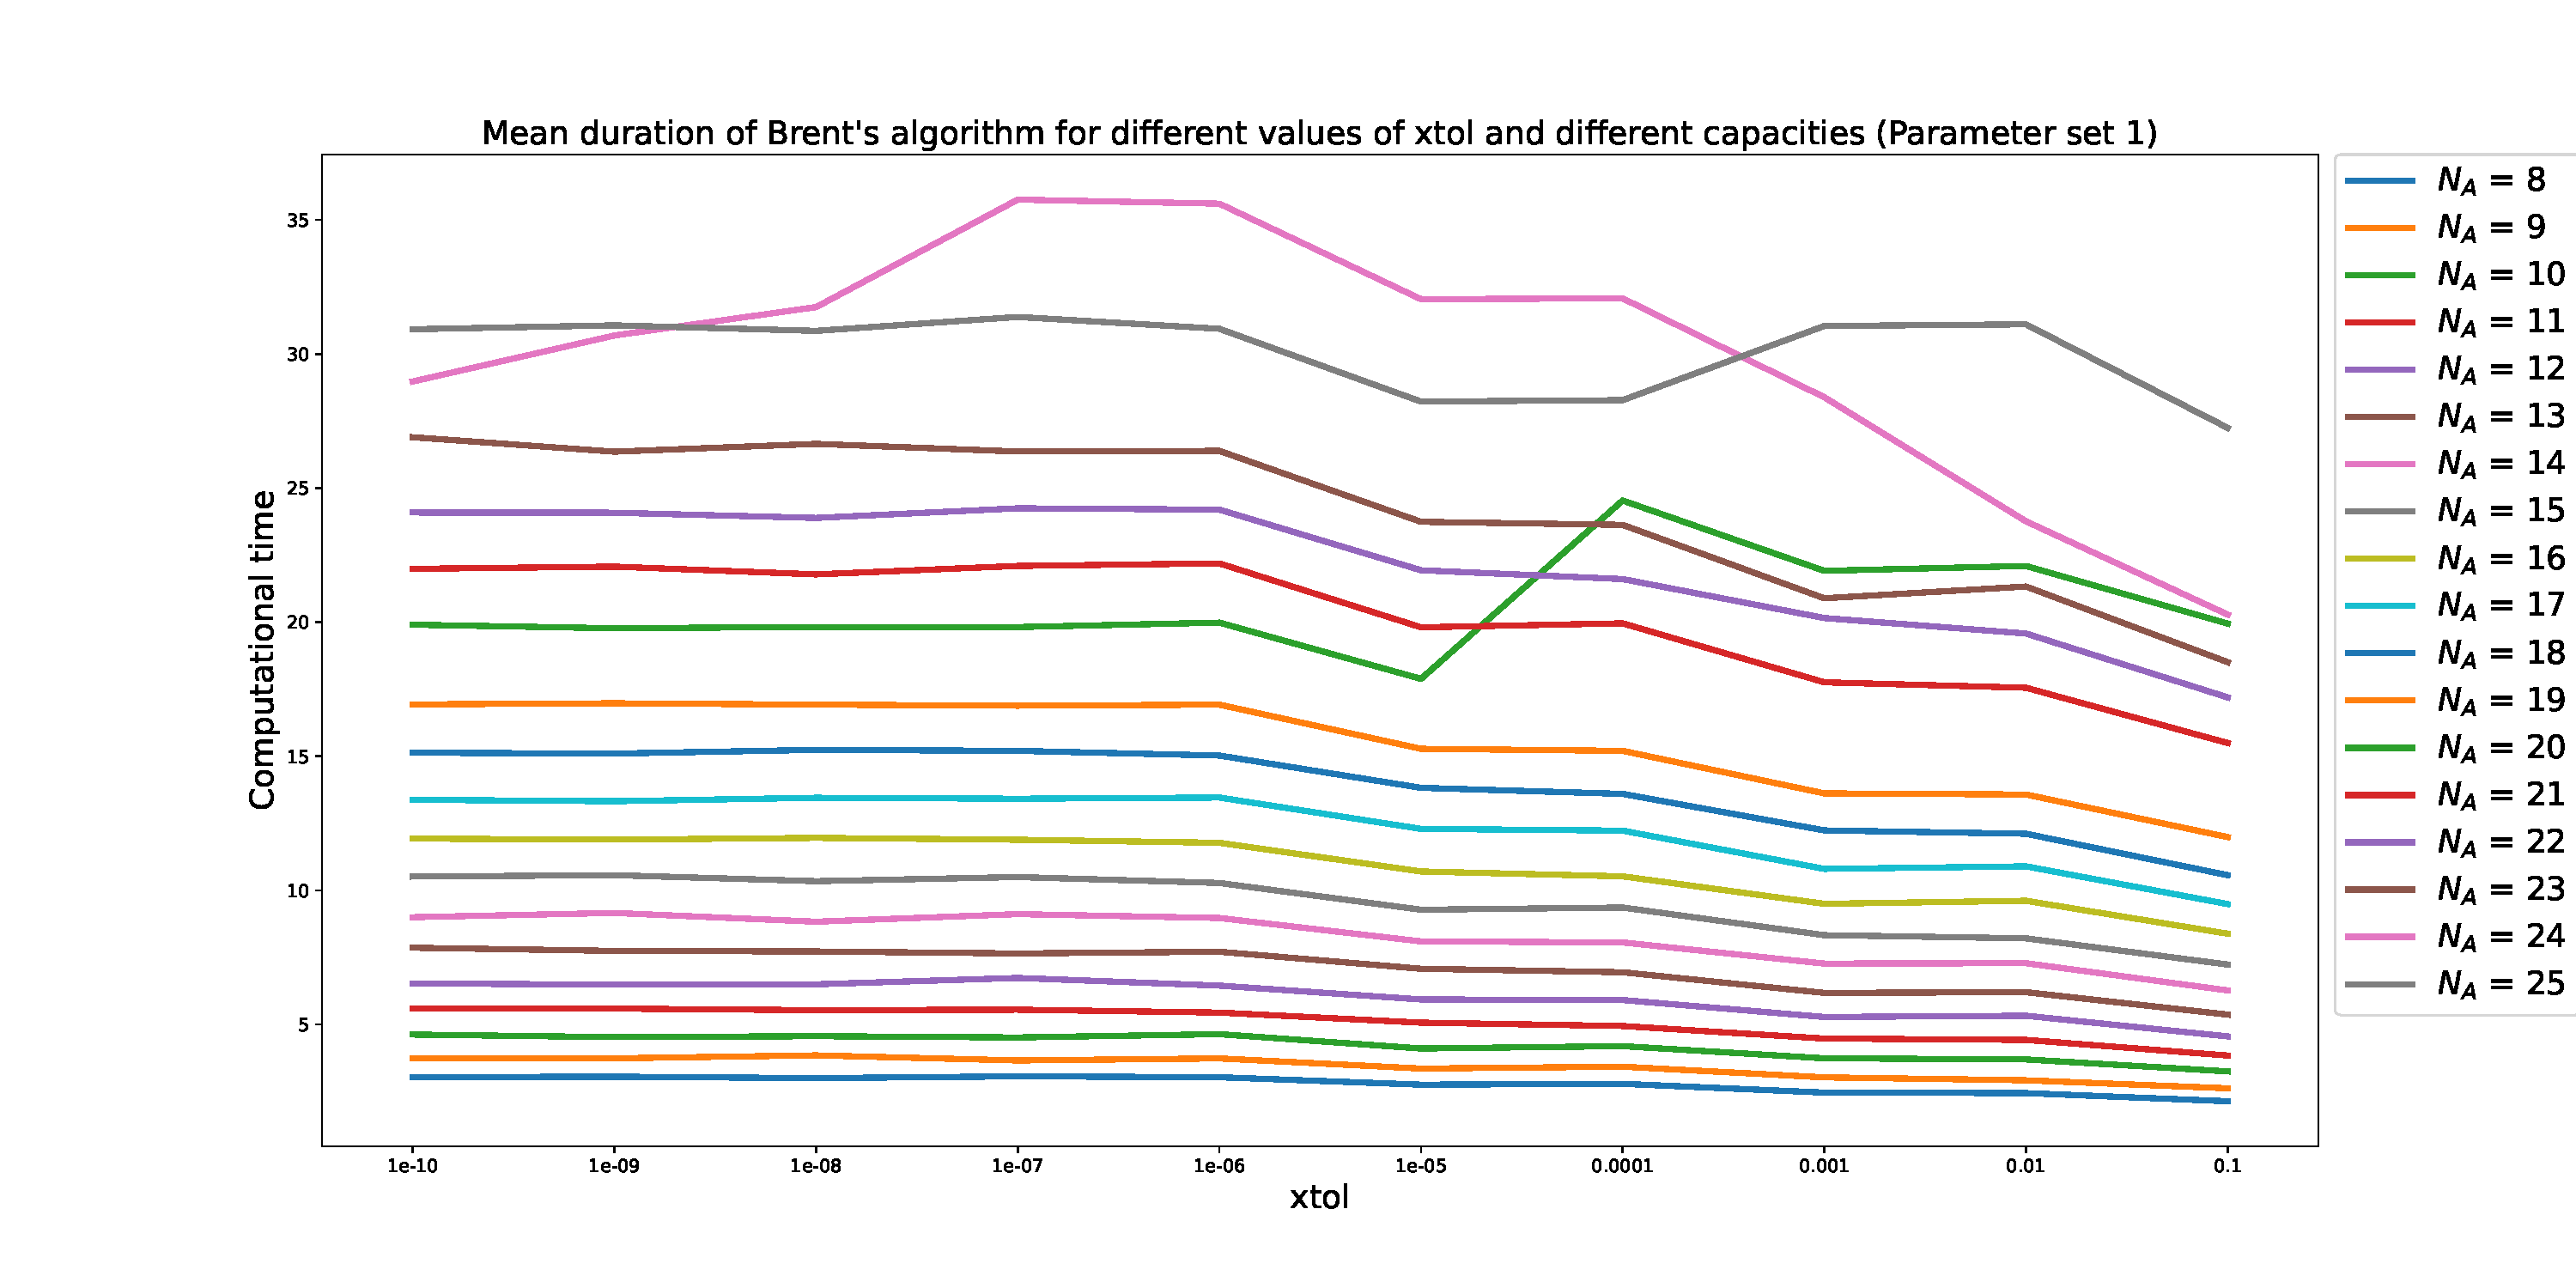
\includegraphics[width=\textwidth]{chapters/04_game_theoretic_model/img/brents_method/tolerance/tolerance_lineplots_1.pdf}
    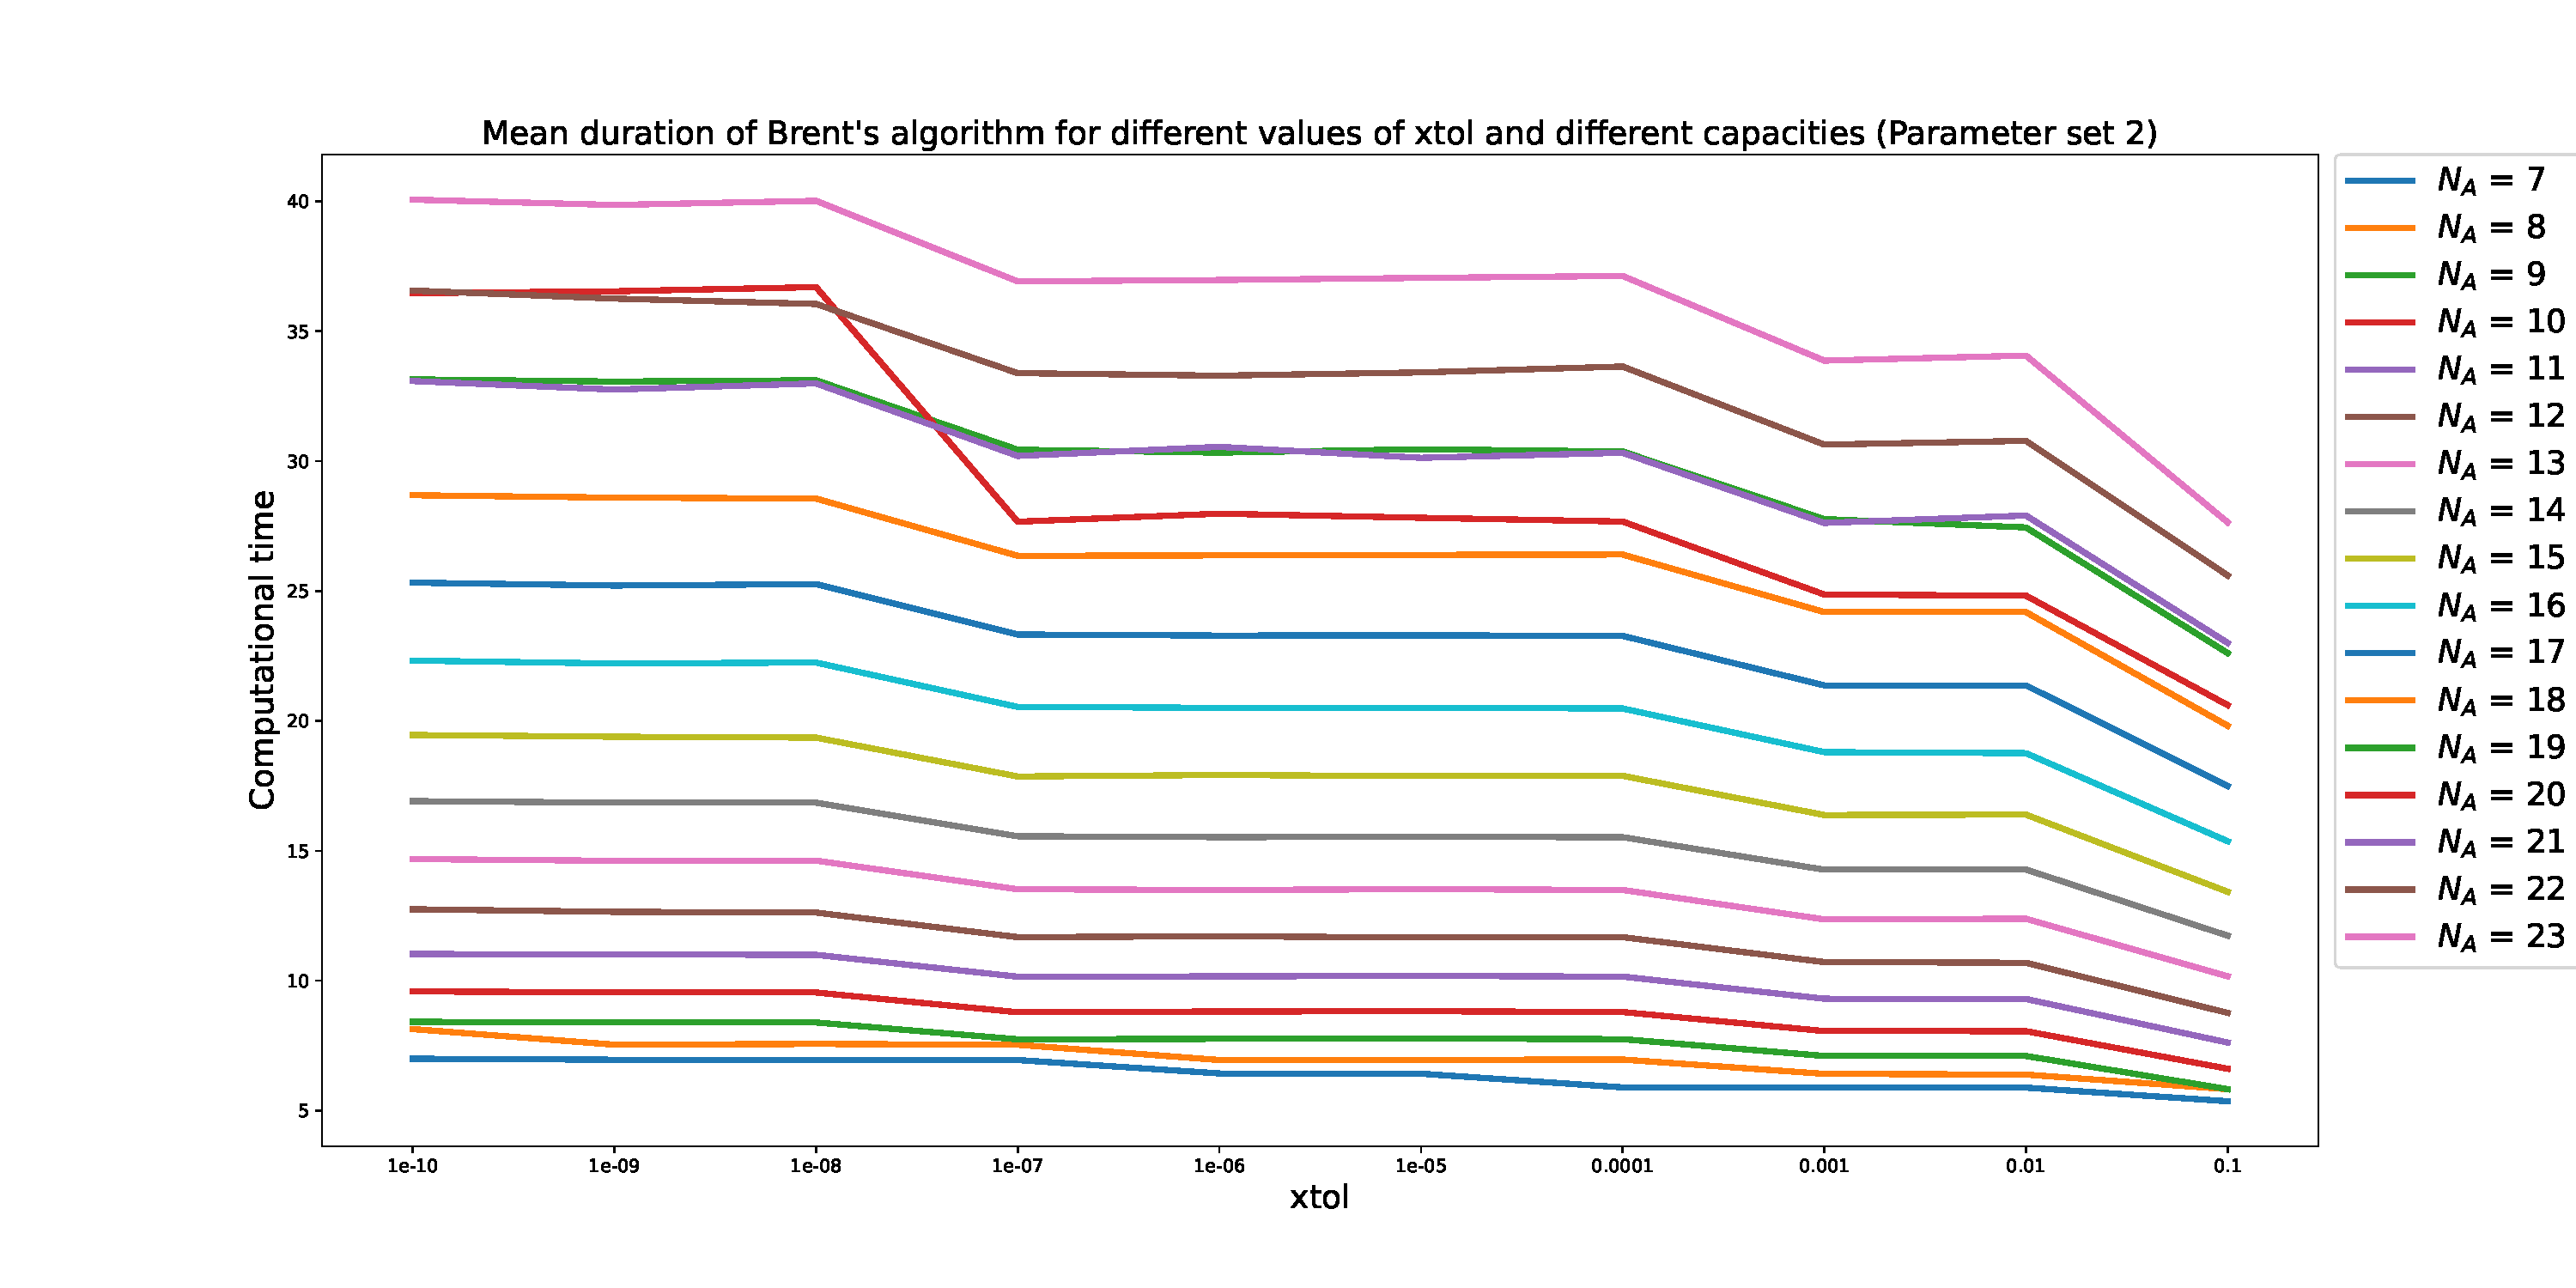
\includegraphics[width=\textwidth]{chapters/04_game_theoretic_model/img/brents_method/tolerance/tolerance_lineplots_2.pdf}
    \caption{
        Line plots of the duration of Brent's method for different values of
        \(N_A\) over different values of the absolute tolerance parameter xtol.
    }
    \label{fig:tolerance_lineplots}
\end{figure}

The plots of Figure~\ref{fig:tolerance_lineplots} show for each value of \(N^A\)
how the duration of the algorithm changes as the absolute tolerance parameter
\lstinline[style=pystyle]{xtol} increases.
It can be seen that for both parameter sets the duration of the algorithm
on most cases the computational time decreases as the tolerance parameter
increases.
There are some cases that do not follow this trend though.
For example, for parameter set 1 when \(N^A=20\), the duration of the algorithm
increases, rather than decreasing, from \lstinline[style=pystyle]{xtol=1e-05}
to \lstinline[style=pystyle]{xtol=0.0001}.



